\documentclass[graybox,envcountchap,twoside,deutsch]{lrt_thesis}
%====================================
% Wenn die Arbeit extern erstellt wird, dann die obige Zeile
% auskommentieren und die nachfolgende Zeile inkludieren:
% \documentclass[graybox,envcountchap,deutsch,extern]{lrt_thesis}
%====================================
\usepackage{etex}
\usepackage[ngerman]{babel}
\usepackage{subfigure}
\usepackage[fleqn]{amsmath}
\usepackage{amsthm,amssymb,amsfonts}
\usepackage[fleqn]{cases}
\usepackage{tabularx}
\usepackage{caption}
\captionsetup{%
  format=hang,
  %indent=1cm,
  font=small,
  justification=justified,
  singlelinecheck=no}
\usepackage{fancyhdr}
\usepackage{multicol}
\usepackage{longtable,booktabs}
%----
\usepackage[numbers]{natbib}
\renewcommand{\bibnumfmt}[1]{#1.}%necessary to achieve correct
                                %formatting of the bib entries
%----
\usepackage{dsfont}
\usepackage[figuresright]{rotating}
\usepackage{ifthen}
\usepackage{trfsigns}
\usepackage[bottom]{footmisc}% places footnotes at page bottom
\usepackage[utf8]{inputenc}
\usepackage{longtable}
%----

%---- By JW ----

%--: Useful Packages :--
\usepackage{listings} % For unformatted Code
\usepackage{float} % Text flow of Pictures

\usepackage[linesnumbered,ruled]{algorithm2e} % For illustrating algorithms
\renewcommand{\algorithmcfname}{Algorithmus}% Update algorithm name

% DRAWING AND STUFF ----------------------------------------------------
\usepackage{tikz} % For drawing
\usepackage{circuitikz} % For Circuit-Drawing
\usepackage[edges]{forest} % For File-Trees
% Some Renewcommands for FOREST-------------------
\definecolor{folderbg}{RGB}{124,166,198}
\definecolor{folderborder}{RGB}{110,144,169}
\newlength\Size
\setlength\Size{4pt}
\tikzset{%
	folder/.pic={%
		\filldraw [draw=folderborder, top color=folderbg!50, bottom color=folderbg] (-1.05*\Size,0.2\Size+5pt) rectangle ++(.75*\Size,-0.2\Size-5pt);
		\filldraw [draw=folderborder, top color=folderbg!50, bottom color=folderbg] (-1.15*\Size,-\Size) rectangle (1.15*\Size,\Size);
	},
	file/.pic={%
		\filldraw [draw=folderborder, top color=folderbg!5, bottom color=folderbg!10] (-\Size,.4*\Size+5pt) coordinate (a) |- (\Size,-1.2*\Size) coordinate (b) -- ++(0,1.6*\Size) coordinate (c) -- ++(-5pt,5pt) coordinate (d) -- cycle (d) |- (c) ;
	},
}
\forestset{%
	declare autowrapped toks={pic me}{},
	pic dir tree/.style={%
		for tree={%
			folder,
			font=\ttfamily,
			grow'=0,
		},
		before typesetting nodes={%
			for tree={%
				edge label+/.option={pic me},
			},
		},
	},
	pic me set/.code n args=2{%
		\forestset{%
			#1/.style={%
				inner xsep=2\Size,
				pic me={pic {#2}},
			}
		}
	},
	pic me set={directory}{folder},
	pic me set={file}{file},
}
%-------------------------------------------------

% Boxes for Datasheet-----------------------------

\usepackage[most]{tcolorbox}

\newtcolorbox{mybox}[2][]{enhanced,
	fonttitle=\ttfamily,
	fontupper=\ttfamily,
	sharp corners,
	colback=white,
	colbacktitle=white,
	coltitle=black,
	boxed title style={colframe=white},
	attach boxed title to top left={yshift=-3mm}, 
	title=#2,#1}

%-------------------------------------------------

% For landscape Tables----------------------------
\usepackage{pdflscape}
\usepackage{afterpage}
%-------------------------------------------------

\usepackage[justification=centering]{caption} % For centering Captions

\usepackage{color, colortbl} % For fancy Tables
\usepackage{booktabs} % For fancy Tables

%--: Code Examples :--
\definecolor{light-gray}{gray}{0.95}
\newcommand{\code}[1]{\colorbox{light-gray}{\texttt{#1}}}

%---------------

%====================================
%Abbreviations
%====================================
\renewcommand{\vec}[1]{\boldsymbol{#1}}

%====================================
%Page layout
%====================================

%------------------------------------
%Geometry
%------------------------------------
\newif\ifmypdf
\ifx\pdfoutput\undefined
  \mypdffalse
  \setlength{\paperwidth}{210mm}
  \setlength{\paperheight}{297mm}
\else
  \mypdftrue
  \usepackage{hyperref}
  \hypersetup{pdftitle={},
    pdfsubject={},
    pdfauthor={Jonas Helmut Wilinski},
    pdfkeywords={RT, Regelungstechnik, Bachelorarbeit, Reinforcement Learning},
    colorlinks=true,
    linkcolor=black,
    citecolor=black,
    plainpages=false,
    a4paper=true,
    plainpages=false,
    pdfpagelabels=true
  }
  \setlength{\paperwidth}{210mm}
  \setlength{\paperheight}{297mm}
\fi

%====================================
%Babel
%====================================
\selectlanguage{ngerman}

%====================================
%Main
%====================================
%
\begin{document}
%
\author{Jonas Helmut Wilinski}
\title{Eine Anwendung des Reinforcement Learning zur Regelung dynamischer Systeme}
\date{September 2018}
\thesistype{Bachelor-Arbeit}
\advisor{Ergänzen} %Nur bei externen Arbeiten (siehe Zeilen 3-5 dieser
                   %Datei)
\examiner{Prof. Dr.-Ing habil. Thomas Meurer}
\abgabedatum{08. September 2018}
\maketitle

%------------------------------------
\fronttitle
\frontmatter
\tableofcontents
\mainmatter
%------------------------------------

%====================================
%  MAIN PARTS
%------------------------------------

\graphicspath{{figures/}}
%
% ****
\chapter*{Abstract und Kurzfassung}
\addcontentsline{toc}{chapter}{Abstract und Kurzfassung}
% ****
%

%
% ***
\section*{Abstract}
% ***
%

English version ... approx. $\frac{1}{2}$ page

%
% ***
\section*{Kurzfassung}
% ***
%

{\Large --- ARBEITSSTAND ---}\vspace{1cm}\\
Diese Bachelorarbeit umfasst den Ansatz, durch \textit{Reinforcement Learning} eine zuverlässige und vergleichbare Regelung von dynamischen Systemen zu erzielen, welche bisher nur durch klassische Regelansätze möglich gewesen ist. Dabei wird im ersten Schritt in Anlehnung an das Tierreich das neuronale Netz des Wurms C. Elegans \cite{WormLevelRL} genauer betrachtet. Der Touch-Withdrawal Circuit ist dafür zuständig, dass das Tier bei Berührung zurückschnellt. Diese Verschaltung der verschiedenen Nervenzellen mittels Synapsen und Gap-Junctions lassen sich exakt nachbilden und mathematisch durch das s.g. \textit{Leaky Integrate and Fire Model} beschreiben.\\
Weiterhin soll ein universeller Simulator zur Implementierung dieses Netzwerkes geschaffen werden, welcher durch zahlreiche Module in der Lage ist, geeignete Parameter zu finden und das Netzwerk auf Probleme der Regelungstechnik anzuwenden. Der Simulator wird dabei in der Programmiersprache \texttt{Python} realisiert und enthält mehrere Dependencies.\\
Ziel dieser Bachelorarbeit ist es, eine verlässliche Regelung dynamischer Systeme als Simulation zu erschaffen und diese mit konventionellen Ansätzen der Regelungstechnik qualitativ zu vergleichen.


%%% Local Variables: 
%%% mode: latex
%%% TeX-master: "main"
%%% End: 

%
% ****
\chapter{Grundlagen der neuronalen Netze}
\label{chap:neuro}
% ****
%
	Dieses Kapitel dient als Einführung in meine Arbeit und zeigt auf, wie im Laufe der Zeit das Konstrukt der neuronalen Netze erforscht und zu Nutze gemacht wurde. Darüber hinaus wird die Notwendigkeit einer Alternative zum klassischen Modell der Rechenmaschine aufgezeigt und genauer beleuchtet. Um die Performance dieser klassischen Automaten bzw. Rechenmaschinen zu testen, werden einige Berechenbarkeitsmodelle vorgestellt. Die einzigartige Umsetzung in Netzwerken neuronaler Nervenzellen ermöglicht es uns, hochkomplexe Aufgaben selbst bei niedrigen Taktfrequenzen durch hohe Parallelität zu bewältigen. Im weiteren Verlauf wird auch auf die Notation und Beschaffenheit neuronaler Netze eingegangen. \\
	Dieser Abschnitt der Bachelorarbeit lehnt sich besonders an die ersten Kapitel der folgenden Bücher an: \textit{R.Rojas - Theorie der neuronalen Netze} \cite{TheorieNeuro} und \textit{Gerstner et al. - Neuronal Dynamics} \cite{NeuronalDynamics}. Weitere Fachartikel werden im Laufe des Kapitels genannt.
% ***
\section{Grundlegende Berechenbarkeitsmodelle}
\label{sec:neuro_models}
% ***
	Im Bereich der Berechenbarkeitstheorie (oder auch Rekursionstheorie) werden Probleme auf die Realisierbarkeit durch ein mathematisches Modell einer Maschine bzw. einem Algorithmus untersucht und kategorisiert. Diese Theorie entwickelte sich aus der mathematischen Logik und der theoretischen Informatik. Neuronale Netze bieten hier eine alternative Formulierung der Berechenbarkeit neben den bereits etablierten Modellen an. Es existieren die folgenden fünf Berechenbarkeitsmodelle, welche durch einen mathematischen oder physikalischen Ansatz versuchen, ein gegebenes Problem zu lösen:
	\begin{itemize}
		\item Das mathematische Modell
			\subitem Die Frage nach der Berechenbarkeit wird in der Mathematik durch die zur Verfügung stehenden Mittel dargestellt. So sind primitive Funktionen und Kompositionsregeln offensichtlich zu berechnen, komplexe Funktionen, welche sich nicht durch primitive Probleme darstellen lassen, jedoch nicht. Durch die \textit{Church-Turing-These}\footnote{Alonzo Church \& Alan Turing, 1936} wurden die berechenbaren Funktionen wie folgt abgegrenzt: "'Die berechenbaren Funktionen sind die allgemein rekursiven Funktionen."'
		\item Das logisch-operationelle Modell (Turing Maschine)
			\subitem Durch die Turing Maschine \footnote{Alan Turing, 1936} konnte neben der mathematischen Herangehensweise an Berechenbarkeitsprobleme eine mechanische Methode eingesetzt werden. Die Turing Maschine nutzte ein langes Speicherband, welches nach gewissen Regeln schrittweise Manipuliert wurde. So konnte sie sich in einer bestimmten Anzahl von Zuständen befinden und nach entsprechenden Regeln verfahren.
		\item Das Computer-Modell
			\subitem Kurz nach dem bahnbrechenden Erfolg von Turing und Church wurden viele Konzepte für elektrische Rechenmaschinen entworfen. Konrad Zuse entwickelte in Berlin ab 1938 Rechenautomaten, welche jedoch nicht in der Lage waren, alle allgemein rekursiven Funktionen zu lösen. Der Mark I, welcher um 1948 an der Manchester Universität gebaut wurde war der erste Computer, welcher alle rekursiven Funktionen lösen konnte. Er verfügte über die damals etablierte Von-Neumann-Architektur\footnote{John von Neumann, 1945} und wurde von Frederic Calland Williams erbaut.
		\item Das Modell der Zellautomaten
			\subitem John von Neumann arbeitete darüber hinaus auch an dem Modell der Zellautomaten, welches eine hoch-parallele Umgebung bot. Die Synchronisation und Kommunikation zwischen den Zellen stellt sich jedoch als herausfordernde Problemstellung heraus, welche nur durch bestimmte Algorithmen gelöst werden kann. Eine solche Umgebung liefert, wenn richtig umgesetzt, eine enorme Rechenleistung dank Multiprozessorarchitektur selbst bei geringen Taktfrequenzen.
		\item Das biologische Modell (neuronale Netze)
			\subitem Neuronale Netze heben sich nun von den vorher beschriebenen Methoden ab. Sie sind nicht sequentiell aufgebaut und können, anders als Zellautomaten, eine hierarchische Schichtenstruktur besitzen. Die Übertragung von Informationen ist daher nicht nur zum Zellnachbarn,  sondern im ganzen Netzwerk möglich. Jedoch wird im neuronalen Netz nicht (wie in der Rechenmaschine üblich) ein Programm gespeichert, sondern es muss durch die s.g. Netzparameter erlernt werden. Dieser Ansatz wurde früher durch mangelnde Rechenleistung der konventionellen Computer nicht weiter verfolgt. Jedoch erfahren wir heute immer mehr den Aufwind neuester Lernalgorithmen und Frameworks, die das Arbeiten im Bereich Deep Learning, Artificial Intelligence und adaptives Handeln unheimlich unterstützen und beschleunigen. Weitergehend ist man heute in der Lage, auf dem Gebiet der Biologie Nervensysteme zu analysieren und von Millionen Jahren der Evolution zu profitieren. So können verschiedene neuronale Netze genauestens beschrieben und simuliert werden.
	\end{itemize}
% ***
\section{Die biologische Nervenzelle}
\label{sec:neuro_nervenzelle}
% ***
	Zellen, wie sie in jeder bekannten Lebensform auftreten, sind weitestgehend erforscht und gut verstanden. Wie alle Zellen im Körper bestehen Sie (stark vereinfacht) aus einer Zellmembran, einem Zellskelett und einem Zellkern, welcher die chromosomale DNA und somit die Mehrzahl der Gene enthält. Sie treten im menschlichen Körper in verschiedenen Größen und mit unterschiedlichen Fähigkeiten auf. Neuronale Nervenzellen wurden über die Evolution dahingehend ausgeprägt, dass sie Informationen Empfangen, verarbeiten und entsenden können. Wie in Abb. \ref{fig:neuron} zu sehen, besteht eine Nervenzelle aus drei Bestandteilen: \textit{Dendrit, Soma und Axom}.
	\begin{figure}[!h] %[!t] ...
		\centering
		\def\svgwidth{12cm}
		\input{figures/chap_neuron/neuron_is.pdf_tex}
		%\includegraphics[width=4cm]{figures/neuron.svg}
		\caption{Schematische Darstellung einer Nervenzelle bestehend aus Dendrit, Soma und Axon.}
		\label{fig:neuron}
	\end{figure}
	\begin{itemize}
		\item Dendrit:
			\subitem Der Dendrit (altgr. 'Baum') dient der Reizaufnahme in der Nervenzelle. Gelangen durch andere Nervenzellen Spannungsspitzen durch vorhandene Synapsen an den Dendrit, leitet dieser die Signale an die Soma weiter.
		\item Soma:
			\subitem Die Zellsoma bezeichnet den allg. Körper der Zelle. Es umfasst den plasmatischen Bereich um den Zellkern, ohne die Zellfortsätze wie Dendriten und Axon. Hier findet der Hauptteil des Stoffwechsels statt, alle ankommenden Signale aus den Dendriten werden integrierend verarbeitet und eine Änderung des Membranpotentials findet statt. Empfangene Signale können erregend oder hemmend auf den Summationsprozess wirken (Siehe Kap. x - LIF Modell). Überschreitet das Membranpotential einen gewissen Threshold, so reagiert die Soma und erzeugt einen Spannungsstoß, welcher an das Axon gegeben wird.
		\item Axon:
			\subitem Das Axon (altgr. 'Achse') ist ein Nervenzellfortsatz, welcher für die Weiterleitung der Signale von der Soma an die Synapsen und damit an andere Nervenzellen verantwortlich ist.
	\end{itemize}
	Verbunden sind Nervenzellen durch s.g. Synapsen, welche den Informationsfluss gewährleisten. Der Informationsfluss geschieht in Synapsen größtenteils chemisch. Bei einem ankommenden Aktionspotential werden Neurotransmitter aus der Zelle ausgeschüttet, welche für einen Ionentransport verantwortlich sind. Nach Übertragung der chemischen Stoffe über den Synapsenspalt werden diese wieder in ein elektrisches Potential umgewandelt. Diese Synapsen treten zwischen benachbarten Nervenzellen bzw. auf kurzer Distanz auf. Elektrische Synapsen hingegen sind noch weitestgehend unerforscht. Sie dienen als Kontaktstellen und ermöglichen eine Übertragung von Ionen und kleineren Molekülen von einer Zelle zur anderen. Die Signalübertragung entfernter Nervenzellen wird somit synchronisiert. Man bezeichnet sie auch als '"Gap-Junctions'". Im weiteren Verlauf dieser Arbeit werden Synapsen nach Abb. \ref{fig:synapse} dargestellt.\\
	\begin{figure}[!h] %[!t] ...
		\centering
		\def\svgwidth{12cm}
		\input{figures/chap_neuron/synapse_is.pdf_tex}
		\caption{Darstellung von verschiedenen Synapsen-Typen.}
		\label{fig:synapse}
	\end{figure}\\
	Bei chemischen Synapsen ist zwischen exzitatorischen und inhibitorischen Synapsen zu unterscheiden. Erstgenannte agieren als erregende Synapsen und übertragen das Aktionspotential mit positivem Vorzeichen an die postsynaptische Nervenzelle. Inhibitorische Synapsen sind hingegen hemmender Natur und führen das Potential mit einem negativen Vorzeichen, sodass es entsprechend negativ gewichtet in den Integrationsprozess der postsynaptischen Nervenzelle eingeht.
% ***
\section{Das biologische neuronale Netz}
\label{sec:neuro_netz}
% ***
	Funktionsweisen neuronaler Netze sind bereits gut erforscht und modelliert worden. Besonders das Nervensystem des Wurms \textit{C. Elegans} \cite{CElegans} ist das bisher am besten verstandene Konstrukt in diesem Bereich der neuronalen Forschung. In dieser Arbeit wird insbesondere auf den s.g. \textit{Touch-Withdrawal-Circuit} eingegangen und versucht, eine Implementierung zu schaffen, welche ein dynamisches System erfolgreich regeln kann.\\
	Ausgangspunkt ist das bereits von Lechner et al. \cite{WormLevelRL} grafisch dargestellte neuronale Netz des C. Elegans, welches den Berührungs-Reflex des Wurms modelliert.
	\begin{figure}[!h] %[!t] ...
		\centering
		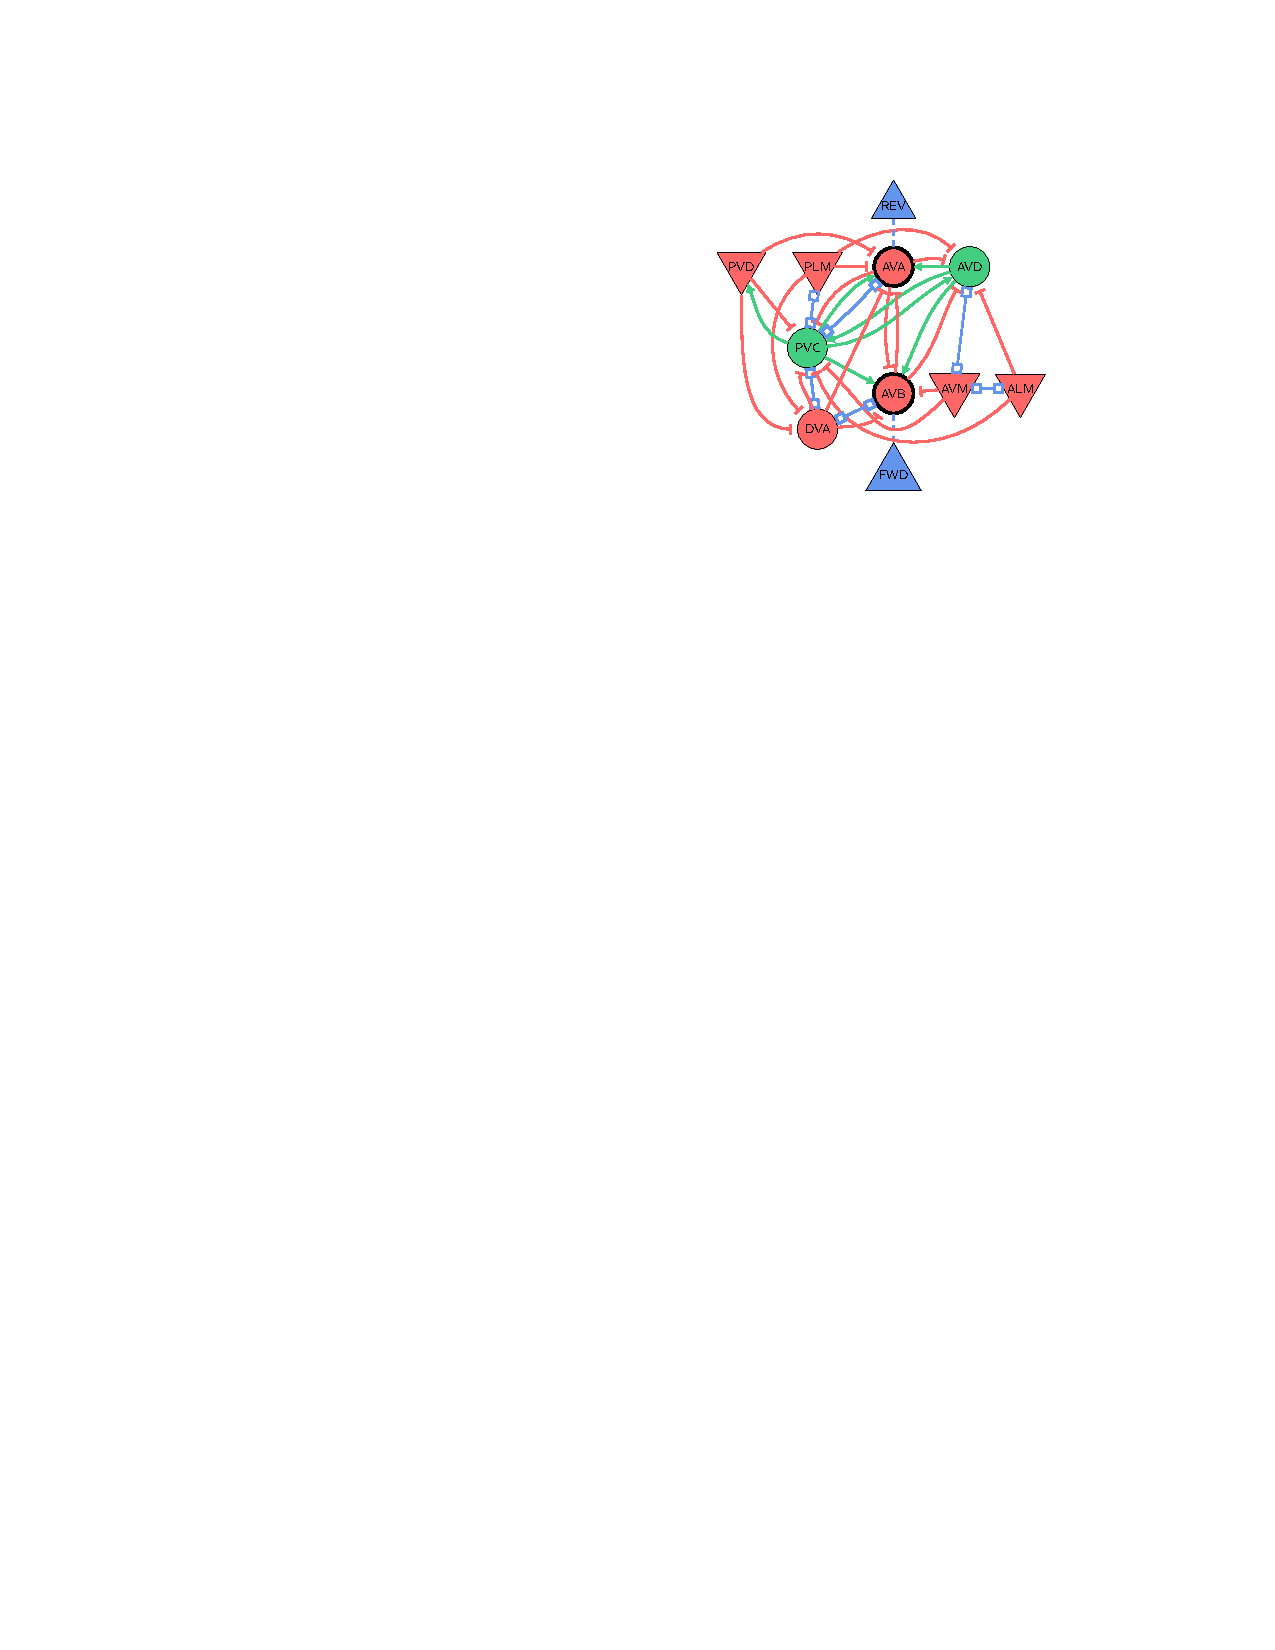
\includegraphics[width=6cm]{figures/chap_neuron/Orig_TW_Circuit.pdf}
		\caption{TW-Neuronal-Circuit nach Lechner et al. \cite{WormLevelRL}}
		\label{fig:01_TW-Circuit}
	\end{figure}
	Wird der Wurm einem äußeren Stimulus - sprich einer Berührung - ausgesetzt, so schnellt er zurück. Anhand des Schaubilds lässt sich nachvollziehen, was in dem Fall einer Berührung in dem neuronalen Netz geschieht:\\
	Die Sensor-Neuronen PVD, PLM, AVM und ALM stellen Rezeptoren dar und reagieren auf Berührung. Sie transduzieren in diesem Fall die Berührung in eine neuronal vergleichbare Form als Aktionspotential und übermitteln diese Information durch die gegebenen Synapsen inhibitorisch oder exzitatorisch an die verbundenen internen Nervenzellen. Dieses Potential beträgt je nach gegebener Intensität der Berührung zwischen $-70mV$ (Ruhespannung - keine Berührung) und $-20mV$ (Spike-Potential - maximale Berührungsintensität) und bildet den Aktionsraum $A\in[-70mV, -20mV]$. Die genannten Sensor-Neuronen lassen sich so beliebig einsetzen und stellen bspw. im Experiment des inversen Pendels positive und negative Observationsgrößen dar. Eine beispielhafte Belegung wäre die folgende:
	\begin{center}
	\begin{tabular}{c@{\hskip 0.5cm}c@{\hskip 0.5cm}c@{\hskip 0.5cm}c}    \toprule
		\setlength{\tabcolsep}{50pt}
		\renewcommand{\arraystretch}{1.5}
		\emph{Umgebungsvariable} & \emph{Typ}  & \emph{Posivite Sensor-Neurone} & \emph{Negative Sensor-Neurone} \\\midrule
		$\varphi$ 				 & Observation & PLM							& AVM							 \\ 
		$\dot{\varphi}$		 	 & Observation & ALM							& PVD							 \\
		$a$						 & Action	   & FWD							& REV							 \\\bottomrule
		\hline
	\end{tabular}
	\end{center}
	Im weiteren Verlauf der Bachelorarbeit werden zudem Vor- und Nachteile aufgezeigt, die genannten Sensor-Neuronen mit anderen Observationsgrößen zu belegen.\\
	Interneuronen, wie PVC, AVD, DVA, AVA und AVB sind direkt mit Sensor-Neuronen sowie untereinander durch Synapsen und Gap-Junctions verbunden. In jeder internen Nervenzelle findet ein Integrationsprozess der jeweiligen anliegenden Ströme aus Stimulus ($I_{Stimuli}$), anderen chemischen Synapsen ($I_{Syn}$) und Gap-Junctions ($I_{Gap}$) statt. Durch das Leaky Integrate and Fire - Modell kann das Membranpotential durch anliegende Ströme zum nächstgelegenen Zeitpunkt bestimmt und ein mögliches Feuer-Event vorhergesagt werden. Eine Nervenzelle feuert ein Signal, wenn das Membranpotential einen Treshold $\theta = -20mV$ erreicht hat. Neurotransmitter werden freigelassen und ein Informationsfluss findet statt.\\
	Um nun den Reflex des Wurms C. Elegans umzusetzen benötigt es noch zwei \textit{Motor-Neuronen}. Diese sind dafür zuständig, ein Befehl in Form eines Feuer-Signals an gewisse Muskelgruppen zu übersetzen, damit diese bewegt werden. In dem behandelten Experiment bedient die Inter-Neurone AVA die Motor-Neurone REV, welche für eine Rückwärtsbewegung steht, analog die Inter-Neurone AVB die Motor-Neurone FWD, welche eine Vorwärtsbewegung initiiert.\\
	Dieser Kreislauf bildet nun ein in sich geschlossenes System mit vier Eingängen und zwei Ausgängen (man achte auf das Mapping mit positiven und negativen Werten) und bildet ein lernfähiges neuronales Netz.
% ***
\section{Das symmetrische neuronale Netz}
\label{sec:my_net}
% ***
	Wie in \cite{Wicks1996} bereits thematisiert, wird in Abb. \ref{fig:01_TW-Circuit} lediglich eine Hälfte des symmetrischen neuronalen Netzes des Wurms C. Elegans beschrieben. Wie im menschlichen Gehirn besteht das Netzwerk aus zwei Hälften, welche zusammenwirken und bei gegebenen Sensor-Input eine Aktion wählen. Eine erweiterte Analyse des Netzwerks besonders mit den berechneten Gewichten der einzelnen Synapsen ergibt, dass das gegebene Netz von Lechner et al. \ref{fig:01_TW-Circuit} unsymmetrisch scheint. Die Nervenzelle \textit{DVA}, welche als Synchronisationszelle zwischen beiden Netzwerkhälften dienen soll, taucht im gegebenen Netz als unsymmetrische Komponente auf und scheint gewisse Sensor-Inputs ungleichmäßig zu gewichten. Im Zuge dessen wird ein neues, symmetrisches neuronales Netz entwickelt, welches zum einen symmetrischer Natur ist, zum anderen manche Synapsen und Gap-Junctions misst, da diese nicht zielführend für das gegebene Problem erschienen. Spätere Simulationen bestätigten diese Annahmen, indem durch Gewichtung der Synapsen und Gap-Junctions manche Verbindungen ein verschwindend geringes Gewicht erhielten.
	\begin{figure}[!h] %[!t] ...
		\centering
		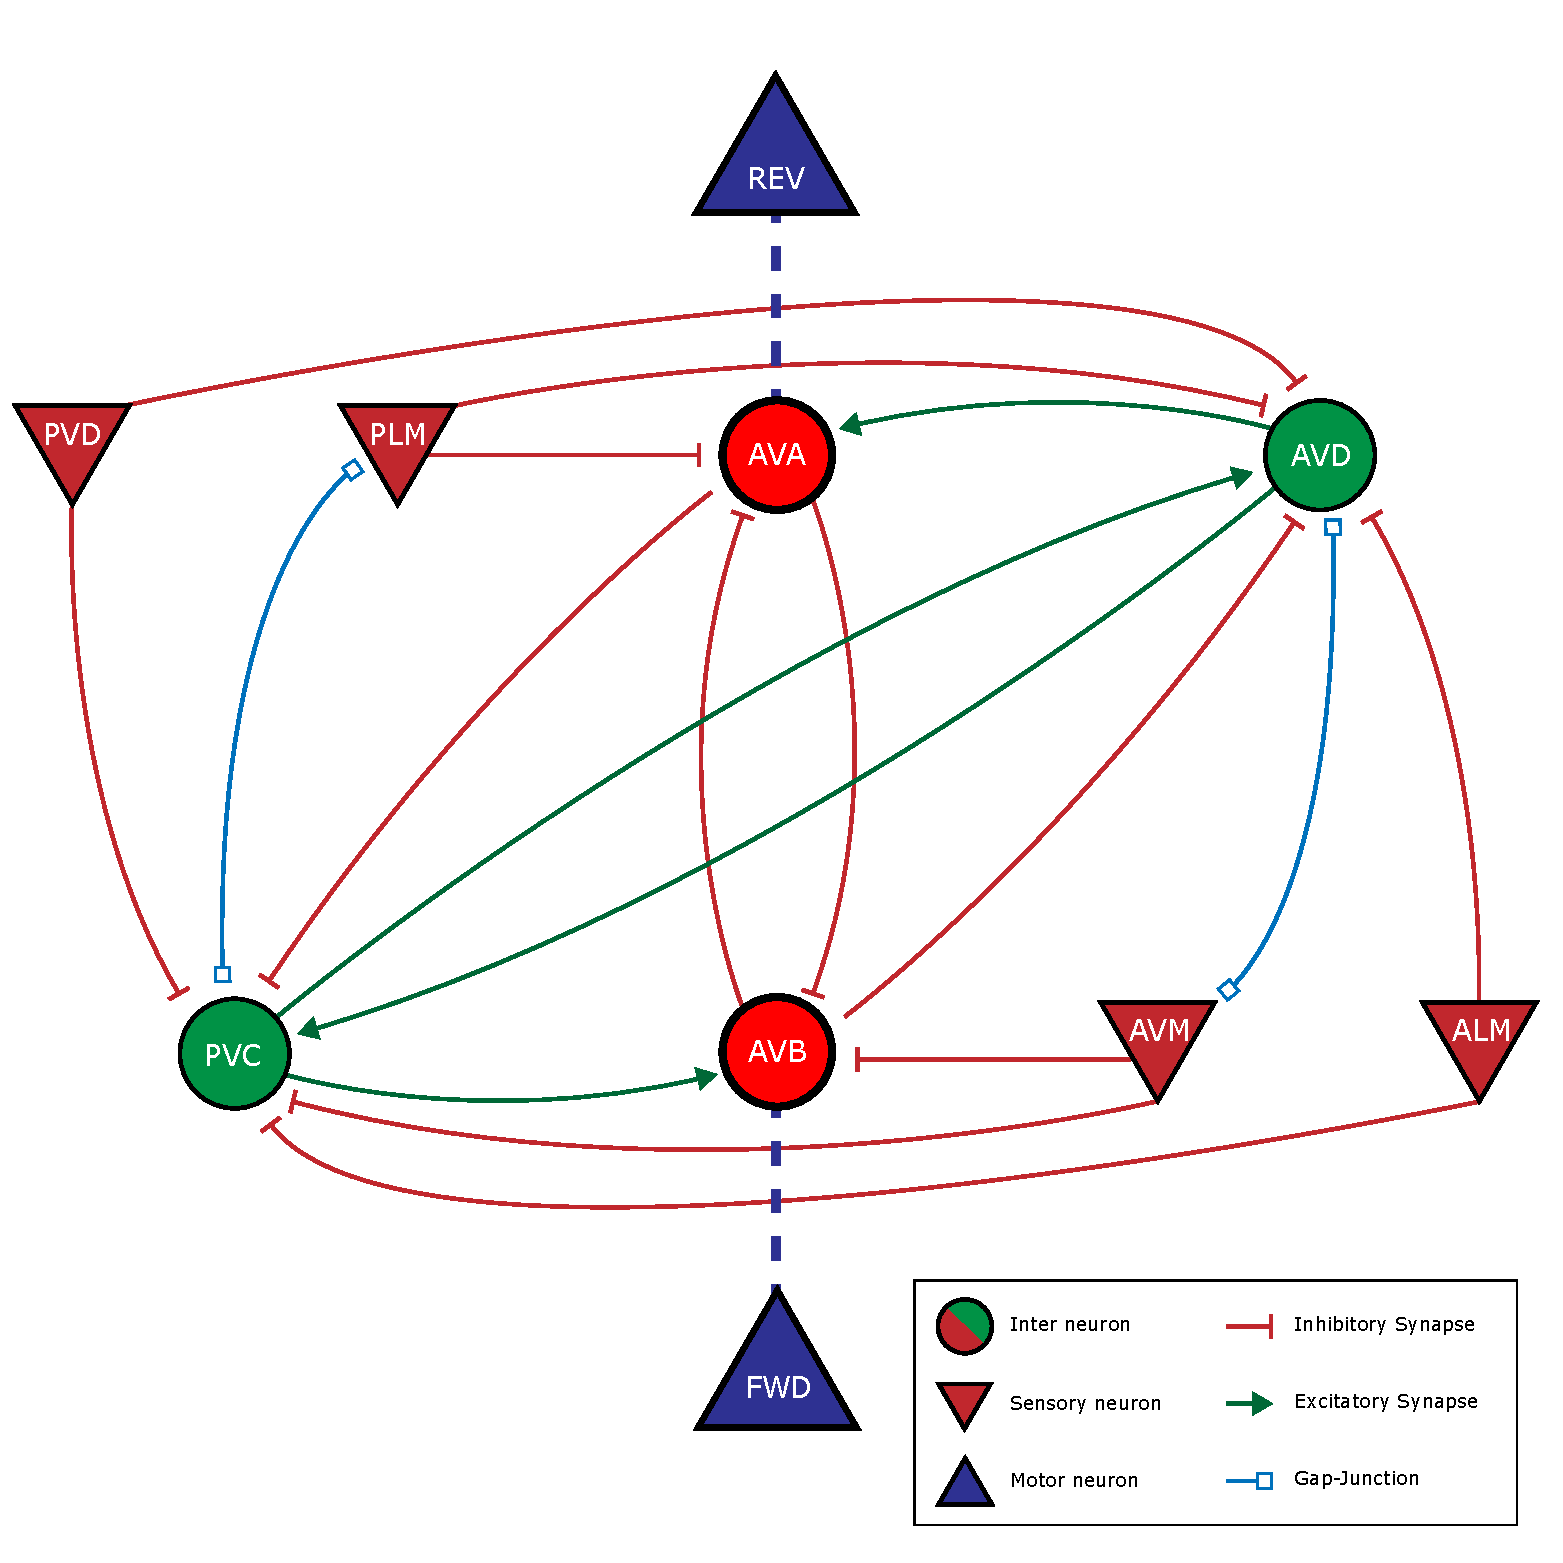
\includegraphics[width=10cm]{figures/chap_neuron/Neural_Net_v3_plain.pdf}
		\caption{Symmetrisches neuronales Netz des TW-Circuits}
		\label{fig:nn_new}
	\end{figure}\\
	Das in Abb. \ref{fig:nn_new} dargestellte, symmetrische neuronale Netz des TW-Circuit wird für alle weiteren Analysen und Simulationsläufe verwendet. Die genaue Umsetzung wird in Kapitel \ref{chap:imp} weiter erläutert.
	

%%% Local Variables: 
%%% mode: latex
%%% TeX-master: "main"
%%% End: 

%
% ****
\chapter{Leaky Integrate and Fire und simulative Modelle neuronaler Netze}
\label{chap:lif}
% ****
%

	Um biologische neuronale Netze zu simulieren und nutzbar zu machen, bedarf es verschiedener Modelle und Algorithmen. Dieses Kapitel stellt das Leaky Integrate and Fire - Modell vor, welches zur Berechnung des Membranpotentials einer internen Nervenzelle dient. Da es sich hier um eine lineare Differenzialgleichung erster Ordnung handelt, werden darüber hinaus numerische Berechnungsmethoden vorgestellt, welche ebenfalls implementiert werden. Weiterhin wird auf die Berechnung der Synapsenströme und Übersetzung der Sensorpotentiale eingegangen und ein simulatives Modell des neuronalen Netzes vorgestellt.

% ***
\section{Das Leaky Integrate and Fire - Modell}
\label{sec:lif_model}
% ***
	Grundsätzlich wird in der Natur beobachtet, dass die neuronale Dynamik als Summationsprozess gefolgt von einer kurzfristigen Entladung des Aktionspotentials beschrieben werden kann. Die Entladung erfolgt hierbei immer ab einem gewissen Wert, welcher als 'Treshold' $\vartheta$ beschrieben wird. Bei Überschreitung 'feuert' die Nervenzelle und Informationen gelangen über Synapsen und Gap-Junctions zu nahegelegenen Neuronen.\\
	Um dieses Verhalten zu modellieren, wird der Zellkern genauer betrachtet. Dieser ist mit einer Zellmembran umgeben, welche als guter Isolator dient. Bei anliegenden Strömen $I_{Stimuli}$, $I_{Syn}$ oder $I_{Gap}$ wird die elektrische Ladung $q = \int I(t')dt'$ die Membran aufladen. Die Zellmembran handelt entsprechend einem Kondensator mit Kapazität $C_m$. Da jedoch in der Natur kein perfekter Kondensator existiert, verliert die Zellmembran über Zeit minimal elektrische Ladung. Daher wird dem Kondensator ein Leckwiderstand $R$ parallel geschaltet. Um das beobachtete Ruhepotential $U_{Leak}$ nach einem Feuer-Event oder bei keinem Input wiederherzustellen, wird eine Batterie in Reihe mit dem Widerstand $R$ geschaltet.\\
	Technisch lässt sich dieses Verhalten als ein elektrisches Ersatzschaltbild wie in Abb. \ref{cic:lif} darstellen (siehe \cite{NeuronalDynamics} Kap. 1.3.1).
	\begin{figure}
		\centering
		\begin{circuitikz}
			\draw	
			%(0,0) to [short, *-*] (5,0)
			(0,4) to [short, o-*] (1,4)
			to [generic, l=$R$] (1,2)
			to [battery1, l=$U_{Leak}$] (1,0)
			to [short, -*] (1,0)
			to [short, -o] (0,0)
			
			(1,4) to [short, i_>=$I(t)$] (3,4)
			to [short, -*] (3,4)
			to [C, l=$C_m$] (3,0)
			to [short, -*] (3,0)
			to [short, -*] (1,0)
			
			(3,4) to [short, -o] (4,4)
			(3,0) to [short, -o] (4,0)
			(4,0) to [open, v_<=$u(t)$] (4,4);
		\end{circuitikz}
		\caption{Ersatzschaltbild der Zellmembran}
		\label{cic:lif}
	\end{figure}
	Um nun eine geeignete Differenzialgleichung herzuleiten, wird zuerst das erste Kirchhoffische Gesetz angewendet
	\begin{align}
		\label{eq:lif_current}
		I(t) = I_R + I_C\text{.}
	\end{align}
	Der erste Strom $I_R$ ist einfach durch das ohmsche Gesetz wie folgt zu berechnen
	\begin{align}
		\label{eq:lif_IR}
		I_R = \frac{U_R}{R} = \frac{U - U_{Leak}}{R}\text{.}
	\end{align}
	Der Strom $I_C$ wird durch die Definition eines Kondensators $C = \tfrac{q}{U}$ zum kapazitiven Strom 
	\begin{align}
		\label{eq:lif_IC}
		I_C = \frac{dq}{dt} = C_m \frac{dU}{dt}\text{.}
	\end{align}
	Hierbei steht $q$ für die elektrische Ladung und $U$ für die anliegende Spannung.\\
	Gleichungen \ref{eq:lif_IR} und \ref{eq:lif_IC} eingesetzt in Gleichung \ref{eq:lif_current} ergibt
	\begin{align}
		\label{eq:lif_I}
		I(t) = \frac{u(t) - U_{Leak}}{R} + C\frac{du}{dt}\text{.}
	\end{align}
	Wird diese Gleichung mit $R$ multipliziert und etwas umgestellt, bildet sich die folgende lineare Differenzialgleichung erster Ordnung:
	\begin{align}
		\label{eq:lif_nd}
		R C \frac{du(t)}{dt} = (U_{Leak} - u(t)) + R I(t)\text{.}
	\end{align}
	Nach Division durch $RC$ und Einführung des Leitwerts $G_{Leak} = \tfrac{1}{R}$ entsteht unsere gewollte Form:
	\begin{align}
		\label{eq:lif}
		\frac{du(t)}{dt} = \frac{G_{Leak}(U_{Leak} - u(t)) + \sum_{i = 1}^{n}{I_{in}}}{C_m}\text{.}
	\end{align}
	In dieser Gleichung stehen die Variablen $G_{Leak}$, $U_{Leak}$ und $C_m$ für Parameter der betrachteten Nervenzelle, während $I(t) = \sum_{i = 1}^{n}{I_{in}}$ stellvertretend für alle eingehenden Ströme aus Stimuli, chemischen Synapsen und Gap-Junctions steht
	\begin{align}
		\label{eq:lif_current}
		I_{in} = I_{Stimuli} + I_{Syn} + I_{Gap}\text{.}
	\end{align}
	Die Implementierung dieser Gleichungen und den entsprechenden nummerischen Lösungsverfahren findet sich in \ref{sec:neuroimp}. Ein beispielhafter Spannungsverlauf bei einem konstanten, positiv einfließendem Strom $I_{in}$ sieht wie folgt aus:
	\begin{figure}[!h]
		\centering
		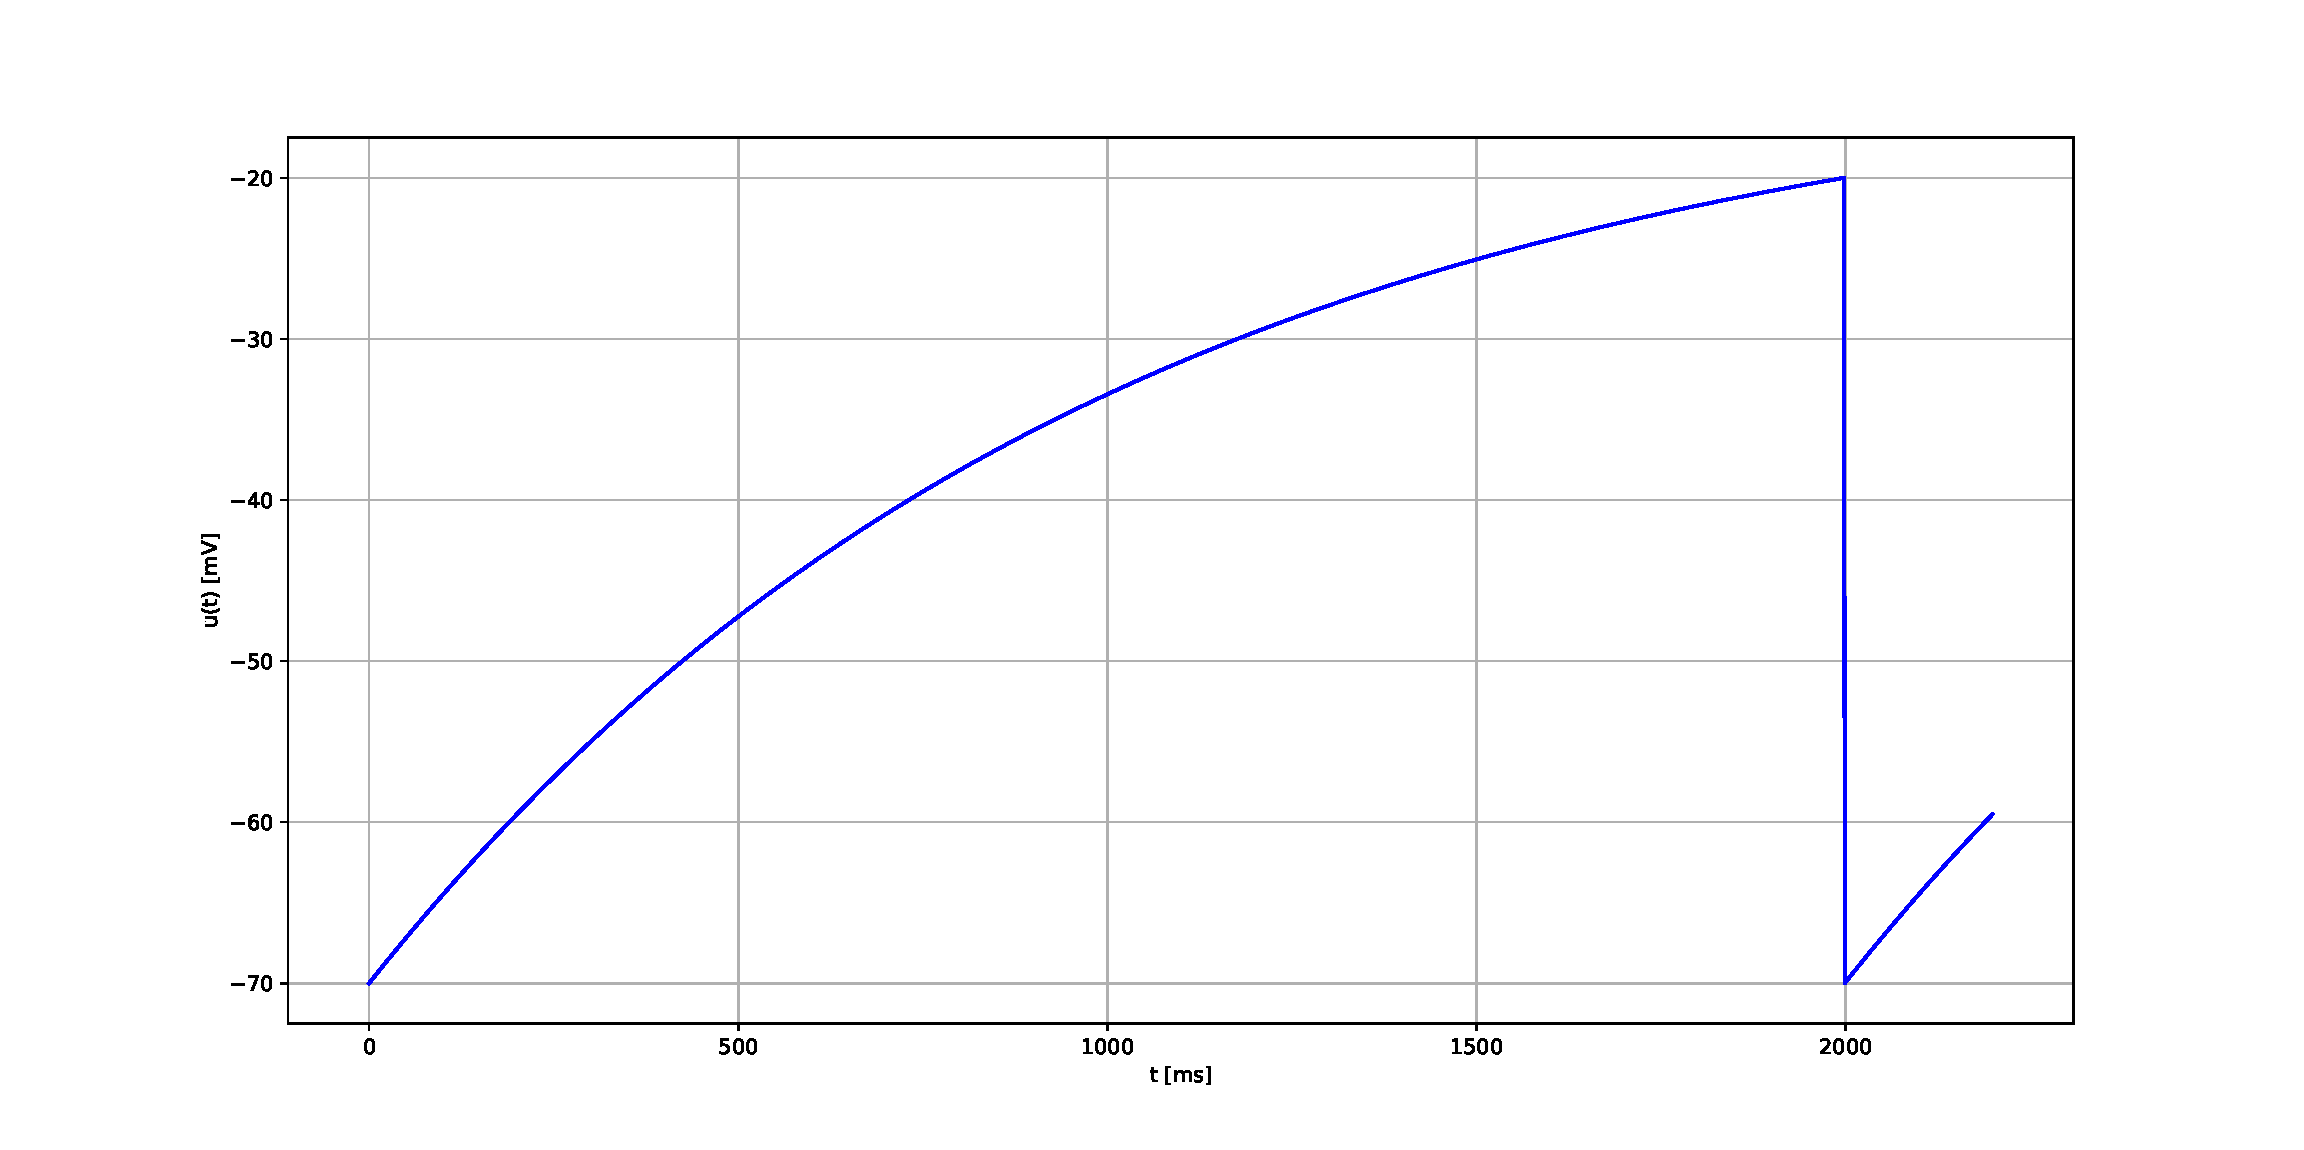
\includegraphics[width=14cm]{figures/chap_lif/Simple_LIF.pdf}
		\caption{Grafische Darstellung des Membranpotentials durch das Leaky Integrate and Fire - Modell}
		\label{fig:simple_lif}
	\end{figure}\\
	Die anliegenden Synapsenströme sind durch folgenden formularen Zusammenhang zu berechnen:
	\begin{align}
		\label{eq:chem_syn_current}
		I_{Syn} = \frac{w}{1 + \e^{\sigma(u_{pre}(t) + \mu)}}(E - u_{post}(t))\text{.}
	\end{align}
	Synapsenströme sind grundsätzlich von den pre- und postsynaptischen Potentialen der jeweiligen Nervenzellen $u_{pre}$ und $u_{post}$ abhängig. Weiterhin können diese chemischen Synapsen exzitatorisch oder inhibitorisch wirken. Diese Eigenschaft wird durch das s.g. Nernstpotential $E\in[0mV, -90mV]$ beschrieben. Weitere Größen dieser Gleichung bilden $w$, die Standardabweichung $\sigma$ und $\mu$.\\
	Gap-Junctions bilden die Ausnahme, denn sie dienen als Ausgleichsglied und wirken bidirektional. Ihr Strom wird wie folgt berechnet:
	\begin{align}
		\label{eq:gap_syn_current}
		I_{Gap} = \hat{w}(u_{post}(t) - u_{pre}(t))\text{.}
	\end{align}
	Für die Berechnung des Gap-Junction Stroms benötigt es ebenfalls das pre und postsynaptische Potenzial der jeweiligen Nervenzellen $u_{pre}$ und $u_{post}$, sowie $\hat{w}$.\\	
	Durch diese formularen Zusammenhänge kann ein ganzheitliches neuronales Netz simuliert werden.
	
% ***
\section{Anwendung auf Modelle neuronaler Netze}
\label{sec:lif_neuro}
% ***
	Durch das im vorherigen Kapitel beschriebene Leaky Integrate and Fire - Modell ist es möglich, interne Vorgänge eines neuronalen Netzes zu beschreiben und zu simulieren. Dies setzt jedoch einen konstanten Input der vier Sensorneuronen durch äußere Stimuli voraus. Diese Rezeptoren sind in der Lage, äußere Einflüsse wie bspw. Licht- oder Berührungsintensität in ein für das neuronale Netz verständliche Größe zu übersetzen. Wie bereits eingangs erwähnt, bewegen wir uns in einem Aktionsraum $A\in[-70mV, -20mV]$, wobei $-70mV$ als Ruhespannung und $-20mV$ als Aktionspotential wahrgenommen wird. Aufgabe der vier Sensor-Neuronen \textit{PVD, PLM, AVM und ALM} ist es folglich, eingehende Größen entsprechend auf den gegebenen Aktionsraum $A$ zu übersetzen.\\
	In dem bereits thematisierten Schaubild nach Lechner et al (Abb. \ref{fig:01_TW-Circuit} \cite{WormLevelRL}) werden jeweils zwei Sensorneuronen für einen Eingang genutzt, da zwischen positiven und negativen Eingangsgrößen unterschieden wird. \textit{PLM und AVM} bilden das primäre Sensorpaar für die ausschlaggebendste Eingangsgröße (inverses Pendel: Winkel $\varphi$), \textit{PVD und ALM} bedienen eine sekundäre Eingangsgröße (inverses Pendel: Winkelgeschwindigkeit $\dot{\varphi}$ oder Cartposition $x$). Diese Wahl beruht auf der internen Verschaltung des Netzwerks durch Synapsen und Gap-Junctions und wird im weiteren Verlauf dieser Arbeit weiter thematisiert.\\
	Um nun die jeweiligen Größen durch die Sensorneuronen zu übersetzen werden folgende Funktionen für die jeweils positive und negative Sensorneurone $S_{positiv}$ und $S_{negativ}$ angenommen:
	\begin{align}
		\label{eq:sensor_translation_p}
		S_{positiv} &:= \begin{cases}-70mV & x\leq 0\\-70mV + \frac{50mV}{x_{min}}x & 0 < x \leq x_{min} \\-20mV & x > x_{max}  \end{cases}\\
		\label{eq:sensor_translation_n}
		S_{negativ} &:= \begin{cases}-70mV & x\geq 0\\-70mV + \frac{50mV}{x_{min}}x & 0 > x \geq x_{min} \\-20mV & x < x_{max}  \end{cases}
	\end{align}
	$x\in[x_{min}, x_{max}]$ ist eine messbare, dynamische Systemvariable, welche in den gegebenen Grenzen $x_{min} $ und $x_{max}$ auftritt. Lediglich eine Fallunterscheidung wird getroffen: nimmt $x$ einen positiven Wert an, wird Sensorneurone $S_{positiv}$ aktiviert, bei negativem $x$-Wert, agiert die Sensorneurone $S_{negativ}$.\\
	Analog lässt sich dieser Zusammenhang auf die beiden Motorneuronen \textit{REV} und \textit{FWD} übertragen. Hier werden die Signale der internen Nervenzellen \textit{AVA} und \textit{AVB} auf interpretierbare Größen in die Außenwelt übersetzt. Biologisch kann dies ein Nervenimpuls sein, welcher eine spezielle Muskelgruppe anspricht oder einen Reflex auslöst. In der hier genannten Simulationsumgebung des inversen Pendels entspricht der Ausgang des Netzwerks entweder einer diskreten Vorwärts- oder Rückwärtsbewegung. Genaueres zu der Interaktion mit dem genannten Simulationskonstrukt im Kapitel \ref{chap:imp}.

% ***
\section{Zuverlässigkeit und Limitationen}
\label{sec:lif_lim}
% ***
	Das Leaky Integrate and Fire - Modell ist stark vereinfacht und zeigt die grundsätzlichen Eigenschaften des Membranpotentials auf. Es erfolgt ein lineares Auf-integrieren der anliegenden Ströme und eine simple Rücksetzung des Aktionspotentials nach Überschreitung des Thresholds $\vartheta$ auf das Ruhepotential $U_{Leak}$.\\
	Zur weiteren Analyse eines neuronalen Netzwerks besonders im Bereich der Biologie und Biochemie werden daher detailliertere Modelle angewendet, um biologische Effekte in verschiedenen Zelltypen zu berücksichtigen. Jedoch eignet sich das hier angewendete Modell sehr gut zur Analyse der gegebenen Nervenzellen. Das Leaky Integrate and Fire - Modell ist in der Lage, s.g. Fire-Events bei der Überschreitung des genannten Thresholds exakt zu ermitteln und liefert somit eine grundlegende Zeitbasis für die Simulationsumgebung.

% ***
\section{Implementierung}
\label{sec:lif_imp}
% ***
	Zur Implementierung des Leaky Integrate and Fire - Modells wird die Programmiersprache \texttt{Python} verwendet. Angelehnt an die Formeln aus \ref{sec:lif_model} kann ein einfacher Algorithmus implementiert werden. Der gesamte Code findet sich in Anhang \ref{sec:lifpy}.\\
	Da sich in der Berechnung der Membranpotentiale eine lineare Differenzialgleichung erster Ordnung ergibt \ref{eq:lif}, muss diese entsprechend numerisch gelöst werden. Die Lösung kann durch das Euler-Verfahren, sowie durch die Methode nach Runge-Kutta gefunden werden, wobei letztere (4. Ordnung) deutlich genauer ist.
	
	\begin{remark}[Numerisches Lösungsverfahren nach Euler]\\
		Gegeben sei eine Differenzialgleichung der Form $\dot{x} = f(x)$ mit der Bedingung $x = x_0$ bei $t = t_0$. Man finde einen Weg, um die Lösung $x(t)$ zu approximieren.\\
		Weiterhin sollte die Schrittweite $\Delta t$ bekannt sein sowie die Anzahl der Zeitschritte $T$. Somit lässt sich die Differenzialgleichung numerisch lösen:
		\begin{align}
			\label{eq:euler}
			x_{n+1} = x_n + f(x_n) \Delta t
		\end{align}
		Aus \cite{NonlinearDynamics}.
	\end{remark}
	\begin{remark}[Numerisches Lösungsverfahren nach erweiterter Euler-Methode]\\
		Gegeben sei ebenfalls eine Differenzialgleichung der Form $\dot{x} = f(x)$ mit der Bedingung $x = x_0$ bei $t = t_0$. Man finde einen Weg, um die Lösung $x(t)$ zu approximieren.\\
		Weiterhin sollte die Schrittweite $\Delta t$ bekannt sein sowie die Anzahl der Zeitschritte $T$. Somit lässt sich die Differenzialgleichung numerisch lösen:
		\begin{align}
			\label{eq:erw_euler}
			\tilde{x}_{n+1} &= x_n + f(x_n) \Delta t\\
			x_{n+1} &= x_n + \tfrac{1}{2}[f(x_n) + f(\tilde{x}_{n+1})]\Delta t
		\end{align}
		Dieses Verfahren ermöglicht eine genauere Approximation als die einfache Euler-Methode bei gleichbleibender Schrittweite. Der Fehler $E = |x(t_n)-x_n|$ wird kleiner. Aus \cite{NonlinearDynamics}.
	\end{remark}
	\begin{remark}[Numerisches Lösungsverfahren nach Runge-Kutta 4. Ordnung]\\
		Gegeben sei eine Differenzialgleichung der Form $\dot{x} = f(x)$ mit der Bedingung $x = x_0$ bei $t = t_0$. Man finde einen Weg, um die Lösung $x(t)$ zu approximieren.\\
		Weiterhin sollte die Schrittweite $\Delta t$ bekannt sein sowie die Anzahl der Zeitschritte $T$. Somit lässt sich die Differenzialgleichung numerisch lösen:
		\begin{align}
			\begin{split}
			\label{eq:runkgekutta}
			k_1 &= f(x_n) \Delta t\\
			k_2 &= f(x_n + \tfrac{1}{2} k_1) \Delta t\\
			k_3 &= f(x_n + \tfrac{1}{2} k_2) \Delta t\\
			k_4 &= f(x_n + k_3) \Delta t\\
			\end{split}\\[10pt]
			x_{n+1} &= x_n + \tfrac{1}{6} (k_1 + 2 k_2 + 2 k_3 + k_4)
		\end{align}
		Dieses Verfahren ermöglicht eine genauere Approximation als die Euler-Methoden bei gleichbleibender Schrittweite. Der Fehler $E = |x(t_n)-x_n|$ wird signifikant kleiner. Diese Methode erfordert jedoch eine höhere Rechenzeit und ist daher nur bei ausreichender Leistung anzuwenden. Aus \cite{NonlinearDynamics}.
	\end{remark}
	Anwendung der Anmerkung 2.3 auf die Funktion \ref{eq:lif} resultiert in folgende Berechnung, welche direkt implementiert werden kann:
	\begin{equation}
	\begin{split}
		\label{eq:runkgekutta_nn}
		k_1 &= \frac{G_{leak} (U_{leak} - u_i(t)) + (I_{Stimuli} + I_{Syn} + I_{Gap})}{C_m} \Delta t\\
		k_2 &= \frac{G_{leak} (U_{leak} - (u_i(t) + \tfrac{1}{2} k_1)) + (I_{Stimuli} + I_{Syn} + I_{Gap})}{C_m} \Delta t\\
		k_3 &= \frac{G_{leak} (U_{leak} - (u_i(t) + \tfrac{1}{2} k_2)) + (I_{Stimuli} + I_{Syn} + I_{Gap})}{C_m} \Delta t\\
		k_4 &= \frac{G_{leak} (U_{leak} - (u_i(t) + k_3)) + (I_{Stimuli} + I_{Syn} + I_{Gap})}{C_m} \Delta t
	\end{split}
	\end{equation}
	Rekursive Berechnung der vier Koeffizienten führt zum neuen Membranpotential und entsprechend zu der Information, ob die internen Nervenzellen \textit{AVA} oder \textit{AVB} gefeuert haben:
	\begin{align}
		\label{eq:runkgekutta_erg}
		u_{i+1}(t) &= u_i(t) + \tfrac{1}{6} (k_1 + 2 k_2 + 2 k_3 + k_4)
	\end{align}
	Um diese Funktion im Gesamtcode später mühelos aufrufen zu können, wird ein Python-Script (\texttt{modules/lif.py}) erstellt. Dieses enthält neben der Funktion zur Berechnung des Membranpotentials auch die der Berechnung von Synapsen- und Gap-Junction-Strömen.\\
	In diversen Such-Algorithmen wird eine Funktion \texttt{compute} implementiert, welche das Modul \texttt{lif.py} aufruft. Um eine effiziente Berechnung der Membranpotentiale und Synapsen- bzw. Gap-Junction Ströme zu gewährleisten, wird die Funktion wie folgt aufgebaut:
	\begin{algorithm}
		\SetKwInOut{Input}{Input}
		\SetKwInOut{Output}{Output}
		
		\Input{$\boldsymbol{x}, \boldsymbol{u}, \boldsymbol{A}, \boldsymbol{B}, \boldsymbol{C_m}, \boldsymbol{G_{Leak}}, \boldsymbol{U_{Leak}}, \boldsymbol{\sigma}, \boldsymbol{w}, \boldsymbol{\hat{w}}$}
		\Output{$\boldsymbol{x}, \boldsymbol{u}, \boldsymbol{fire}, \boldsymbol{I_{Syn}}, \boldsymbol{I_{Gap}}$}
		
		\For{i $\leftarrow$ 1 \textbf{to} 4}{
			\For{j $\leftarrow$ 1 \textbf{to} 4}{
				\uIf{$\boldsymbol{A_{i,j}} == 1$}{
					I\_inter$_{i,j}$ = I\_syn\_calc($x[i], x[j], E_{in}, w[k], \sigma[k], \mu$)\\
					k $\leftarrow$ k + 1
				}
				\uElseIf{$\boldsymbol{A_{i,j}} == 2$}{
					I\_inter$_{i,j}$ = I\_syn\_calc($x[i], x[j], E_{ex}, w[k], \sigma[k], \mu$)\\
					k $\leftarrow$ k + 1
				}
				\Else{
					I\_inter$_{i,j}$ = 0
				}
			
				\uIf{$\boldsymbol{B_{i,j}} == 1$}{
					I\_sensor$_{i,j}$ = I\_syn\_calc($u[i], u[j], E_{in}, w[k], \sigma[k], \mu$)\\
					l $\leftarrow$ l + 1
				}
				\uElseIf{$\boldsymbol{B_{i,j}} == 3$}{
					I\_sensor$_{i,j}$ = I\_gap\_calc($u[i], x[j], \hat{w}[k]$)\\
					m $\leftarrow$ m + 1
				}
				\Else{
					I\_sensor$_{i,j}$ = 0
				}
			}
		}
		\For{i $\leftarrow$ 0 \textbf{to} 4}{
			I\_inter = I\_inter.sum(axis = 0)\\
			I\_sensor = I\_sensor.sum(axis = 0)\\
			x[i], fire[i] = U\_neuron\_calc($x[i], I\_inter[i], I\_sensor[i], C_m[0,i], G_{Leak}[0,i], U_{Leak}[0,i], v, \Delta t$)
			
		}
		\KwRet{$\boldsymbol{x}, \boldsymbol{u}, \boldsymbol{fire}, \boldsymbol{I_{Syn}}, \boldsymbol{I_{Gap}}$}
		\caption{compute}
	\end{algorithm}
	Die Vektoren $\boldsymbol{x}$ und $\boldsymbol{u}$ spiegeln die aktuellen Membranpotentiale der jeweiligen Nervenzellen wieder:
	\begin{align}
		\boldsymbol{x} &= \begin{pmatrix}AVA & AVD & PVC & AVB\end{pmatrix}\text{ und}\\
		\boldsymbol{u} &= \begin{pmatrix}PVD & PLM & AVM & ALM\end{pmatrix}\text{.}
		\label{eq:xu}
	\end{align}
	Vektor $\boldsymbol{x}$ beschreibt das Membranpotential interner Nervenzellen, Feuer-Events der Neuronen \textit{AVA} und \textit{AVB} sind später von Interesse. $\boldsymbol{u}$ stellt das Potential für die Eingangsneuronen dar, welche durch die Berechnungsvorschriften \ref{eq:sensor_translation_p} und \ref{eq:sensor_translation_n} je nach Sensordaten gesetzt werden.\\
	Matrizen $\boldsymbol{A}$ und $\boldsymbol{B}$ werden als Transitionsmatrizen genutzt, um die Verbindungen der Neuronen im neuronalen Netz zu beschreiben.
	\begin{align}
		\boldsymbol{A} &= \bordermatrix{
		\quad\Rsh& AVA & AVD & PVC & AVB \cr
			AVA &  0  &  0  &  1  &  1  \cr
			AVD &  2  &  0  &  2  &  0  \cr
			PVC &  0  &  2  &  0  &  2  \cr
			AVB &  1  &  1  &  0  &  0  \cr
		}
	\end{align}
	beschreibt Verbindungen innerhalb der internen Nervenzellen. Dabei stehen die Ziffern $[0,1,2]$ für folgende Verbindungen:
	\begin{align*}
		0 &: \text{Keine Verbindung zwischen Neuronen }\boldsymbol{A_i}\text{ und } \boldsymbol{A_j}\\
		1 &: \text{Inhibitorische Verbindung zwischen Neuronen }\boldsymbol{A_i}\text{ und }\boldsymbol{A_j}\\
		2 &: \text{Exzitatorische Verbindung zwischen Neuronen }\boldsymbol{A_i}\text{ und }\boldsymbol{A_j}.
	\end{align*}
	Die Matrix
	\begin{align}
	\boldsymbol{B} &= \bordermatrix{
		\quad\Rsh& AVA & AVD & PVC & AVB \cr
			PVD &  0  &  1  &  1  &  0  \cr
			PLM &  1  &  1  &  3  &  0  \cr
			AVM &  0  &  3  &  1  &  1  \cr
			ALM &  0  &  1  &  1  &  0  \cr
		}\text{.}
	\end{align}
	beschreibt analog die Verbindungen der Sensor-Neuronen mit den internen Nervenzellen. Verbindungen werden zwischen diesen Typen von Nervenzellen nur durch inhibitorische Synapsen und Gap-Junctions gemacht. Die Ziffern $[0,1,3]$ haben folgende Bedeutung:
	\begin{align*}
		0 &: \text{Keine Verbindung zwischen Neuronen }\boldsymbol{B_i}\text{ und } \boldsymbol{B_j}\\
		1 &: \text{Inhibitorische Verbindung zwischen Neuronen }\boldsymbol{B_i}\text{ und }\boldsymbol{B_j}\\
		3 &: \text{Verbindung durch Gap-Junction zwischen Neuronen }\boldsymbol{B_i}\text{ und }\boldsymbol{B_j}.
	\end{align*}

%%% Local Variables: 
%%% mode: latex
%%% TeX-master: "main"
%%% End: 


% ****
\chapter{Reinforcement Learning - Lernen mit Belohnung}
\label{chap:rl}
% ****
%

	Reinforcement Learning (kurz: RL) kann als einer der drei großen Bereiche des Maschine Learning interpretiert werden. Neben den Bereichen \textit{Supervised-} und  \textit{Unsupervised Learning} deckt es ein weites Spektrum an Anwendungsfeldern ab.
	
	Die grundsätzliche Vorgehensweise im Reinforcement Learning ist simpel: Ein Agent ist in der Lage, eine Simulation oder ein Spiel zu bedienen. Seine Aktion beeinflusst eine gut bekannte Umwelt bzw. Simulationsumgebung. Die Ergebnisse dieser Aktion werden durch das Beobachten der Umwelt bzw. der Simulation interpretiert und eingeschätzt. Der Lernprozess erfolgt, indem der Agent durch die Interpretierung der Observation und einer Belohnung eine Aktion tätigt, welche diese maximieren soll. Durch die immer größer werdende Datenbasis fällt es dem Agenten mit fortgeschrittener Simulation immer leichter, die \glqq richtigen\grqq{} Aktionen zu treffen, um die maximale Belohnung zu erhalten.
	

% ***
\section{Reinforcement Learning - eine Abwandlung des Deep Learning}
\label{sec:rl_dl}
% ***
	Deep Learning hat in den letzten Jahren immer mehr an Relevanz gewonnen. Obwohl der Grundstein dieser Algorithmen und Vorgehensweisen bereits Ende des 19. Jahrhunderts gelegt wurde, fehlte es damals sowohl an Rechenleistung, als auch an hoch parallelen Rechenstrukturen. In der Theorie ist das Konstrukt des Deep Learning in der Lage, bei gegebenen Berechnungsmodellen mit multiplen verbundenen Ebenen Strukturen in großen Datenmengen zu erkennen. Durch heute verfügbare Rechenleistungen können Strukturen ein beliebig hohes Abstraktionslevel aufweisen. Anwendungsbereiche für Deep Learning bewegen sich meist im Bereich der Bild- oder Spracherkennung und Klassifizierung, breiten sich jedoch auch auf weitere Bereiche wie Medizin (Pharmazie, Genom-Entschlüsselung) oder Wirtschaft (Kunden-Kaufverhalten, Logistik) aus. Dabei zeichnet einen guten Deep Learning Algorithmus die Fähigkeit aus, sog. Raw-Files (unbearbeitete Signale wie bspw. Audio-Dateien oder Bilder) ohne Vorwissen auf die gewünschten Daten zu untersuchen und zu klassifizieren, ohne aufwendige Filter, Feature-Vektoren oder andere Mittel zur Vorklassifikation.
	
	\textit{Supervised Learning} (zu Deutsch: überwachtes Lernen) bildet die Grundlage und wurde in den Anfängen der künstlichen Intelligenz eingesetzt. Ein Algorithmus lernt aus gegebenen Paaren von Ein- und Ausgängen eine Funktion, welche nach mehrmaligen Trainingsläufen Assoziationen herstellen soll und auf neue Eingaben passende Ausgaben liefert \cite{DeepLearning}.
	
	\textit{Unsupervised Learning} (zu Deutsch: unüberwachtes Lernen) bietet entgegen der Methode des supervised Learning die Möglichkeit, ein Modell ohne im Voraus bekannte Zielwerte oder Belohnungssysteme durch die Umwelt zu trainieren. Entsprechend benötigen diese Algorithmen mehr Rechenleistung (bei gleichbleibender Aufgabenstellung). Sie versuchen, in einer Anhäufung von Datenstrukturen zu erkennen, welche von stochastischem Rauschen abweichen. Neuronale Netze orientieren sich hier oft an den bekannten Eingängen. Diese Methode wird oft in Bereichen der automatischen Klassifizierung oder Dateikomprimierung genutzt, da hier das Ergebnis im Vorhinein meist unbekannt ist \cite{DeepLearning}.
	
	\textit{Reinforcement Learning} bietet, wie bereits in der Einleitung erwähnt, den Vorteil eines Belohnungssystems.
	\begin{figure}[H] %[!t] ...
		\centering
		\def\svgwidth{12cm}
		\input{figures/chap_rl/RL_Chart.pdf_tex}
		\caption{Graphische Darstellung des Reinforcement Learning Algorithmus.}
		\label{fig:rl_chart}
	\end{figure}
	Der Agent beginnt mit einer anfangs willkürlich gewählten Aktion und beeinflusst damit die Umwelt bzw. die Simulation. Durch einen Interpreter ist es möglich, wichtige Messgrößen (inverses Pendel: Winkel $\varphi$ oder Winkelgeschwindigkeit $\dot{\varphi}$) zu messen und in einen Observationsvektor $\textbf{o}$ zu schreiben. Dieser kann ausgelesen werden und den aktuellen Zustand $x$ nach der erfolgten Aktion liefern. Dazu wird durch ein anfangs definiertes Lohn-System eine vereinbarte Belohnung geliefert, welcher die Performance der Simulation widerspiegelt. Der Agent besitzt nun diese Informationen und entscheidet aufgrund des gegebenen Zustandes sowie der Belohnung, welche Aktion als nächstes getätigt werden soll. In der Theorie wird so die Belohnung mit jeder erfolgreichen Episode höher und der Agent ist in der Lage gewisse Parameter der Simulation entsprechend des jeweiligen Observationsparameters anzupassen.
	
	Bei dieser Methode ist die Grundlage aller Algorithmen und Optimierungsverfahren der Gesamtreward
	\begin{align}
		G_t = \sum_{k=0}^{T}R_{t+k+1}.
	\end{align}
	Des Weiteren ist es geläufig, einen sog. \glqq Discount-Faktor\grqq{} $\gamma$ einzuführen. Belohnungen in frühen Schritten der Simulation sind wahrscheinlicher und gut vorherzusehen, wohingegen in fortgeschrittenen Simulationen die Aktionen meist schwer vorhersehbar sind und somit eine höhere Belohnung verdienen.
	\begin{align}
		G_{t\gamma} = \sum_{k=0}^{\infty}\gamma^k R_{t+k+1}\text{ mit }\gamma\in[0,1)
	\end{align}
	Von der Benutzung eines solchen Discount-Faktors wird jedoch vorerst abgesehen, da das Finden der perfekten Parameter für die vorgestellte Simulation im Vordergrund steht. In weiteren Anwendungen kann dieser Faktor eingeführt werden.
	
% ***
\section{Anwendung auf Modelle neuronaler Netze}
\label{sec:rl_neuro}
% ***
	Reinforcement Learning findet klassischerweise Anwendung durch Deep Learning Algorithmen auf künstlich erstellten neuronalen Netzen mit vielen s.g. \glqq Hidden Layers\grqq{} (Ebenen zwischen Ein- und Ausgang mit hoher Anzahl an Neuronen) statt. Variiert werden in einem solchen Netz lediglich die jeweiligen Gewichte der Synapsen zwischen den Neuronen. Synapsen sind darüber hinaus einfache Mittel zur Informationsübertragung und haben keine weiteren Eigenschaften oder zeigen kein eigenes Verhalten.
	
	Das hier vorliegende neuronale Netzwerk ist jedoch gänzlich anders aufgebaut. Nervenzellen werden durch Potenziale beschrieben und integrieren anliegende Informationen auf. Synapsen können verschiedener Art sein und entsprechend hemmend sowie erregend wirken. Sowohl Nervenzellen als auch Synapsen (und Gap-Junctions) haben verschiedene Parameter, welche gewisse Aktionen im neuronalen Netz verursachen können.
	
	Daher wird die Methode des Reinforcement Learning auf biologische neuronale Netze abgewandelt, um diese auf Probleme der Regelungstechnik anzuwenden. Folglich befassen wir uns mit einem neuronalen Netz, welches eine Ebene mit vier Neuronen aufweist. Diese  arbeiten wie bereits in Kapitel \ref{chap:neuro} und \ref{chap:lif} beschrieben ebenfalls anders als in den üblichen Modellen künstlicher neuronaler Netze.
	
	Die Schwierigkeit dieser Aufgabenstellung besteht darin, geeignete Parameter für jede Nervenzelle sowie für jede Synapse und Gap-Junction zu finden, sodass das Netz korrekt und zuverlässig auf interpretierte Signale aus der Umwelt reagiert und entsprechend durch den Agenten eine Aktion wählt, welche eine möglichst hohe Belohnung nach sich zieht. Bezogen auf Abbildung \ref{fig:rl_chart} stellt die Umwelt unsere Simulationsumgebung des inversen Pendels (\texttt{OpenAI Gym - CartPolev0}) dar. Diese nimmt eine Aktion (FWD oder REV) pro Simulationsschritt an und gibt entsprechend einen Observationsvektor $\textbf{o}$ aus, welcher durch den Interpreter übersetzt wird. Der aktuelle Zustand $x$ wird durch die vier Sensorneuronen \textit{PVD, PLM, AVM} ud \textit{ALM} entsprechend interpretiert und in das neuronale Netz eingegeben.

% ***
\section{Verschiedene Suchalgorithmen}
\label{sec:rl_alt}
% ***
	Die Wahl des geeigneten Suchalgorithmus ist immer von der Beschaffenheit der Problemstellung abhängig. Klassische Probleme mit Anwendung des Reinforcement Learning auf künstliche neuronale Netze nutzen Algorithmen wie Q-Learning, Policies (Epsilon-Greedy, Gradient-Decend und -Acend) oder genetische Algorithmen. Diese sind hoch spezialisiert und suchen nach Maxima der gegebenen Funktion, um den Fehler zu reduzieren. Bei einer großen Zahl an Parametern, welche untereinander noch korreliert sein können, kommt oft der einfache, jedoch gleichzeitig sehr effektive \glqq Random-Search\grqq{} Algorithmus zum Einsatz.
	
	Grundsätzlich sei noch zu erwähnen, dass konventionelle Such- bzw. Optimierungsalgorithmen innerhalb des Reinforcement Learning ein Markov-Entscheidungsproblem voraussetzen. 
	\subsection{Q-Learning}
	\label{subsec:rl_qlearning}
		Die Methode des Q-Learnings wurde zuerst von Watkins \cite{Watkins1992} definiert und vorgestellt. Voraussetzung um diese Algorithmen anzuwenden ist eine kontrollierte Markov Umgebung.
		\begin{remark}[Markow Eigenschaft und Umgebung]
			Als Markow-Eigenschaft\footnote{Nach Andrei Markow (1856 - 1922)} bezeichnet man, wie stark ein stochastischer Prozess von der eigenen Vergangenheit abhängt. Diese Bedingung erlaubt es, Markow-Prozesse zu beschreiben.
			
			Durch eine Markow-Umgebung ist es möglich, aus einer begrenzten Anzahl an vergangenen Zuständen die Wahrscheinlichkeit für das Eintreten zukünftiger Ereignisse durch selbst gewählte Aktionen vorherzusagen. \cite{SilverRL}
		\end{remark}
		Ziel der Q-Learning Methode ist es, die Qualität der getätigten Aktionen bei unterschiedlichen Simulationsbedingungen zu verbessern. Dabei wird ein Agent eingesetzt, welcher lernt, in einer Markow-Umgebung optimal zu handeln, indem die Konsequenzen der Aktionen sofort zurückgeführt, analysiert und verarbeitet werden. Dem Agenten ist zu jedem Zeitpunkt der Simulation die Umwelt unbekannt.
		
		Unmittelbar nach einer getätigten Aktion $a$ erhält der Agent neben dem Zustand $x$ (ausgwählte Messgrößen wie bspw. der Winkel des inversen Pendels $\varphi$) die Belohnung $R_x(\pi(x))$. Aus diesen Informationen lässt sich der Wert $V^\pi$ des erhaltenen Zustandes $x$ berechnen:
		\begin{align}
			V^\pi(x) \equiv R_x(\pi(x)) + \gamma \sum_{y}P_{xy}[\pi(x)]V^\pi(y)
		\end{align}
		mit $\gamma$ als Diskontierungsfaktor der nächsten Belohnung und $P_{xy}$ als Wahrscheinlichkeit der nächsten vorhergesagten Veränderung der Umwelt.
		
		Nach Watkins existiert mindestens eine optimale stationäre Vorgehensweise (\glqq Policy\grqq) $\pi^*$ für welche gilt
		\begin{align}
			V^*(x) \equiv V^{\pi^*}(x) = \max_{\substack{a}} \bigg\{R_x(a) + \gamma \sum_{y}P_{xy}[a]V^{\pi^*}(y)\bigg\}.
		\end{align}
		Ziel des sog. \glqq Q-Learner\grqq{} ist es, diese optimale Vorgehensweise zu finden. So lassen sich die charakteristischen Q-Values
		\begin{align}
			Q^\pi(x,a) = R_x(a) + \gamma \sum_{y}R_{xy}[\pi(x)]V^\pi(y)
		\end{align}
		berechnen. Diese spiegeln die erwartete, diskontierte Belohnung bei Ausführung einer Aktion $a$ mit Zustand $x$ und der darauf folgenden Vorgehensweise $\pi$ wieder. Zusammenfassend kann durch die Methode des Q-Learning eine optimale Vorgehensweise des Agenten erzielt werden, wenn die entsprechenden Q-Values der optimalen Vorgehensweise gefunden bzw. erlernt werden.
	\subsection{Gradient Policies}
		Eine weitere Möglichkeit, Probleme durch Reinforcement Learning zu lösen, ist die Anwendung sog. \glqq Gradient Policies\grqq{}. Dies stellt ein klassisches Optimierungsproblem dar und fordert in erster Linie ebenfalls eine Markow-Umgebung.
		
		Es wird eine gegebene Vorgehensweise $\pi_\theta(x,a)$ mit Parametern $\theta$ angenommen. Ziel ist es, die optimalen Parameter $\theta$ zu finden, um die Belohnung zu maximieren. Um die Qualität der Vorgehensweise $\pi_\theta$ zu messen, wird
		\begin{align}
			J(\theta) = V^{\pi_\theta}(x)
		\end{align}
		als Qualitätsgröße abhängig von der gegebenen Vorgehensweise sowie dem Zustand $x$ eingeführt. Policy Gradient Algorithmen suchen nach einem lokalen Maximum in $J(\theta)$, indem sie sich entlang des Gradienten der Vorgehensweise 
		\begin{align}
			\Delta \theta = \alpha \nabla_\theta J(\theta)
		\end{align}
		bewegen. $\alpha$ ist dabei ein Schrittweitenparameter.	Somit ist $\nabla_\theta J(\theta)$ definiert als
		\begin{align}
			\nabla_\theta J(\theta) = \begin{pmatrix}
			\frac{\partial J(\theta)}{\partial \theta_1} & \\
			\vdots & \\
			\frac{\partial J(\theta)}{\partial \theta_n} & \end{pmatrix}.
		\end{align}
		Bei Anwendung von Gradient Policies stellt sich eine gute Konvergenzeigenschaft des Lernalgorithmus ein. Durch das stetige Bewegen auf dem erlernten Gradienten der Qualitätsgröße $J(\theta)$ wird ein Maximum gefunden. Jedoch spiegelt dieses lediglich ein lokales Maximum wider und ist mit geringer Wahrscheinlichkeit gleichzeitig ein globales Optimum. Darüber hinaus bietet sich die Methode bei großen Aktionsräumen und langen Laufzeiten an, da selbst stochastische Prozesse erlernt werden können. \cite{SilverRL} 
	\subsection{Genetische Algorithmen}
	\label{subsec:gen_alg}
		Die Anwendung genetischer Algorithmen im Bereich des Reinforcement Learning ist ebenfalls schon seit einiger Zeit bekannt und führt in den richtigen Situationen zu zufriedenstellenden Ergebnissen.
		
		Der Grundstein dieser Optimierungsverfahren wurde von Holland et al. in seinem Werk \glqq Adaption in Natural and Artificial Systems\grqq{} \cite{Holland1992} gelegt. Basierend auf den bereits von Darwin\footnote{Charles Darwin (1809 - 1882)} beobachteten Phänomenen der Natur, setzen genetische Algorithmen bei dem Ansatz \glqq Survival of the Fittest\grqq{} an. Grundsätzlich kann die Vorgehensweise genetischer Algorithmen wie folgt dargestellt werden \cite{Goldberg1989}:
		\begin{itemize}
			\item Die erste Generation an Parametern wird zufällig initialisiert. Gleich der RandomSearch Methode werden über eine Gleichverteilung verschiedene Parameter erzeugt.
			\item Es werden Simulationen mit den Parametern der ersten Generation gefahren. Die entsprechende Güte wird anhand des Rewards festgelegt.
			\item Durch eine festgelegte Grenze werden Kandidaten der ersten Generation mit sehr guten Parametern selektiert, welche zur Rekombination genutzt werden
			\item Die Rekombination kann als eine Aktualisierung der Parametergrenzen verstanden werden.
			\item Durch Mutation werden anhand der neuen Parametergrenzen erneut zufällige Parameter erzeugt. Diese werden wieder durch Simulation evaluiert und sollten in der Theorie nun bessere Ergebnisse erzielen.
			\item Noch einmal erfolgt eine Selektion basierend auf neuen Auswahlkriterien der Mutationen.
		\end{itemize}
		Die Schritte der Selektion, Rekombination, Mutation und Evaluierung werden bis zu einem gewählten Abbruchkriterium durchlaufen.
		\begin{figure}[H] %[!t] ...
			\centering
			\def\svgwidth{12cm}
			\input{figures/chap_rl/gen_alg.pdf_tex}
			\caption{Graphische Darstellung des genetischen Algorithmus.}
			\label{fig:gen_chart}
		\end{figure}
		Wie in Abbildung \ref{fig:gen_chart} anschaulich dargestellt, verringert sich mit jeder Generation der Parameterraum und die Simulation konvergiert optimaler Weise zu einem globalen Maximum. Dieses hängt jedoch stark von der Anzahl der Selektionen sowie der gewählten Varianz bei Mutation ab. Hier ist ein optimaler Trade-Off zwischen Rechenleistung und Simulationsdauer zu finden.
		
		Wie nachfolgend in Kapitel \ref{chap:imp} beschrieben findet die Anwendung genetischer Algorithmen auf das vorgestellte biologische Netzwerk statt.
	\subsection{Random-Search}
		Gewisse Probleme in der Domäne des Reinforcement Learning erfordern einen verallgemeinerten Ansatz zum Finden von optimalen Parametern. Das hier vorliegende Problem bietet eine große Anzahl an lokalen Maxima und bereitet daher den meisten Algorithmen Probleme bei der Anwendung. Ein Anpassen an die geforderten Umstände ist im Grunde möglich, erfordert jedoch einen hohen Rechenaufwand und führt evtl. zu keiner Verbesserung der Ergebnisse. Daher wird die Methode des Random Search angewendet.
		
		Ähnlich zum genetischen Algorithmus werden Parameter für die Simulation in vorher festgelegten Grenzen durch eine Gleichverteilung erzeugt. Diese werden auf eine Simulation angewendet und die Performance wird anhand der Belohnung ausgewertet. Durch ein simples High Score System werden Parameter mit guter Belohnung gespeichert, schlechte Simulationen werden verworfen. Durch den Einsatz von genügend Rechenleistung und langen Simulationszeiten können so sehr gute Parameter gefunden werden (siehe Appendix \ref{app:parameter}).
	
	Wie im vorherigen Abschnitt \ref{sec:rl_neuro} bereits kurz beschrieben, werden die jeweiligen Parameter der Synapsen und Nervenzellen gesucht. Dies sind die folgenden:
	\begin{table}[H]
		\centering
		\resizebox{0.9\columnwidth}{!}{%
		\begin{tabular}{l@{\hskip 0.5cm}c@{\hskip 0.5cm}c@{\hskip 0.5cm}c}    \toprule
			\setlength{\tabcolsep}{50pt}
			\renewcommand{\arraystretch}{1.5}
			\emph{Parameter-Typ} 	& \emph{Parameter}  & \emph{Beschreibung} 				& \emph{Grenzen} 					 \\\midrule
			Membranpotential		& $C_m$				& Kapazität der Zellmembran			& $[1\text{ mF}, 1\text{ F}]$						 \\ 
			Membranpotential	 	& $G_{Leak}$		& Leitwert der Zellmembran			& $[50\text{ mS}, 5\text{ S}]$						 \\
			Membranpotential	 	& $U_{Leak}$		& Ruhepotential der Zellmembran		& $[-90\text{ mV}, 0\text{ mV}]$						 \\
			Synapsenstrom			& $E_{Excitatory}$	& pos. Beeinflussung des Membranpotentials	& $[0\text{ mV}]$							 \\
			Synapsenstrom			& $E_{Inhibitory}$	& neg. Beeinflussung des Membranpotentials		& $[-90\text{ mV}]$							 \\ 
			Synapsenstrom			& $\mu$				& Erwartungswert (Modelle)			& $[-40\text{ mV}]$							 \\
			Synapsenstrom			& $\sigma$			& Standardabweichung (Modell)		& $[0.05, 0.5]$						 \\ 
			Synapsenstrom		 	& $w$				& Kreisfrequenz der Synapsen		& $[0\text{ S}, 3\text{ S}]$							 \\
			Synapsenstrom			& $\hat{w}$			& Kreisfrequenz der Gap-Junctions	& $[0\text{ S}, 3\text{ S}]$							 \\\bottomrule
			\hline
		\end{tabular}}
		\caption{Grenzen der essentiellen Parameter im biologischen neuronalen Netz.}
		\label{tab:rl_parameter}
	\end{table}
	Die gegebenen Grenzen folgen aus \cite{WormLevelRL} und \cite{SimCE} und sind durch Calcium und Potassiummengen im Nervensystem des \textit{C. Elegans} verbunden.

%%% Local Variables: 
%%% mode: latex
%%% TeX-master: "main"
%%% End: 

%
% ****
\chapter{Implementierung des TW-Netzes}
\label{chap:imp}
% ****
%

	\begin{minipage}[b]{0.65\textwidth}
		Die Implementierung des gesamten neuronalen Netzes inklusive der Simulationsumgebung erfolgt in der Programmiersprache \texttt{Python}. Als Module werden zum einen das bereits vorgestellte Leaky Integrate and Fire - Modell implementiert, zum anderen diverse Algorithmen zur Suche von individuellen Parametern des neuronalen Netzes. Darüber hinaus ist das Programm in der Lage, eine Simulation der gefundenen Parameter durch die Simulationsumgebung \texttt{CartPole\_v0} von OpenAI Gym zu zeigen und Parameter über die Simulationszeit zu plotten. Die Module sowie diverse Dokumentationen und Informationen sind in meinem GitHub-Repository\footnotemark{} zu finden. Ein entsprechendes Deckblatt mit weiteren Informationen liegt dieser Arbeit in Anhang \ref{app:parameter} bei.
	\end{minipage}
	\begin{minipage}[b]{0.35\textwidth}
		\begin{figure}[H] %[!t] ...
			\centering
			
\includegraphics[width=5cm]{figures/appendix/qr-code.pdf}
			\caption{QR-Code Verweis zum GitHub-Repository.}
			\label{fig:qr}
		\end{figure}
	\end{minipage}
	\footnotetext{https://github.com/J0nasW/BA}
		

% ***
\section{Aufbau des Programms}
\label{sec:imp_module}
% ***
	Ein Ziel dieser Arbeit ist es, neben der Funktionstüchtigkeit des Simulators das entstandene Programm mitsamt allen Modulen und Abhängigkeiten modular und leicht verständlich aufzubauen. Dazu gehört eine gute Dokumentation sowie saubere Versionierung, um Änderungen nachvollziehbar darzustellen.\\
	Folgende Anforderungen werden an das Programm gestellt:
	\begin{itemize}
		\item Es existiert ein zentraler Punkt zum Ändern aller nötigen Parameter. Alle weiteren Größen werden durch Formeln und Abfragen erzeugt.
		\subitem Datei: \texttt{parameters.py}
		\item Es wird ein Modul zur Visualisierung gegebener Parameter oder Gewichte des neuronalen Netzes bereitgestellt. Diese Datei muss leicht verständlich und manipulierbar sein, um eigene Plots zu erstellen und neue Simulationsumgebungen einzubinden.
		\subitem Datei: \texttt{visiualize.py}
		\item Es muss die Möglichkeit bestehen, aus bereits existierenden Suchalgorithmen neue Implementationen zu erstellen und gegebene Funktionen einfach einsetzen zu können.
		\subitem Vorlage: \texttt{random\_search\_v2.py}, \texttt{weights\_nn.py}, \texttt{genetic\_algorithm.py}
	\end{itemize}
	Aufgrund der hohen Vielfältigkeit an neuronalen Netzen und Suchalgorithmen soll dieses Programm als Basis für neue Projekte und Ideen dienen. Daher wird empfohlen, eine Fork des Repositories (siehe Anhang \ref{app:parameter}) zu erstellen und den Simulator weiter zu gestalten.\\
	Das Programm beinhaltet folgende Module:\\
	\begin{minipage}{0.35\textwidth}
		\vspace{0.3cm}
		\begin{forest}
			pic dir tree,
			where level=0{}{% folder icons by default; override using file for file icons
				directory,
			},
			[TW Circuit
				[docs]
				[information]
				[modules
					[genetic\_algorithm.py, file]
					[inspect.py, file]
					[lif.py, file]
					[parameters.py, file]
					[random\_search\_v2.py, file]
					[visiualize.py, file]
					[weights.py, file]]
				[parameter\_dumps]
				[weight\_dumps]
				[main.py, file]]
		\end{forest}
	\end{minipage}
	\begin{minipage}{0.65\textwidth}
		\begin{itemize}
			\item Der Ordner \texttt{docs} beinhaltet wichtige Dokumentationen bezüglich des Codes und dem Umgang mit diversen Befehlen innerhalb der \texttt{main.py}. Darüber hinaus wird hier ebenfalls diese Arbeit inklusive des \LaTeX-Codes abgelegt.
			\item Aufgrund vieler komplexer Simulationen mit verschiedenen Parametersätzen wurde die Berechnung von Heim- und Unirechnern auf Rechenzentren ausgelagert. Der Ordner \texttt{information} wird genutzt, um Informationen über jede Simulation (Ergebnisse, Zeitstempel, Zugehörigkeit, ...) in Form einer TXT-Datei zu speichern.
			\item Alle nötigen Module zur Simulation und Visualisierung finden sich in dem Ordner \texttt{modules} wieder. Genauere Informationen zu den einzelnen Skripten werden in den nächsten Sektionen aufgeführt.
			\item parameter\_dumps und weight\_dumps sind die Resultate der Simulationsläufe. In diesen Ordnern werden Parameter und Gewichte des neuronalen Netzes nach erfolgreichen Simulationsläufen abgespeichert. Die Dateien werden durch das Skript \texttt{hickle} in ein HDF-5 Dateiformat \cite{hdf5} gespeichert.
		\end{itemize}		
	\end{minipage}
	
	
		
% ***
\section{Implementierung der Suchalgorithmen}
\label{sec:imp_search}
% ***
	Die Suchalgorithmen befinden sich jeweils in dem Ordner \texttt{modules} und werden durch Import in der Datei \texttt{main.py} aufgerufen. Sie erhalten bei Aufruf die vom Anwender gewählte Simulationszeit (bspw. 12 Stunden) und bei Bedarf bereits errechnete Parameter. Als Ausgabe wird ein Dump der errechneten Parameter oder Gewichte gespeichert sowie eine Informationsdatei, welche Zugehörigkeiten, Anz. an Simulationen, Laufzeiten und den gesamten Reward beschreibt. 
	
	\subsection{Suchalgorithmus RandomSearch}
		Der Suchalgorithmus RandomSearch wurde direkt in die Simulation eingebunden. Es werden die Parameter $C_m, G_{Leak}, U_{Leak}, \sigma, w, \hat{w}$ durch eine Gleichverteilung in den bereits genannten Grenzen zufällig erzeugt. Um gleich-verteilte, zufällige Werte zu generieren, wird die Funktion \texttt{random.uniform} aus dem bekannten Package \texttt{numpy} \cite{NumPy} verwendet.
		\begin{algorithm}
			\SetKwInOut{Input}{Input}
			\SetKwInOut{Output}{Output}
			
			\Input{Anz. Nervenzellen, Anz. Synapsen, Anz. Gap-Junctions}
			\Output{Arrays $\boldsymbol{C_m, G_{Leak}, U_{Leak}, \sigma, w, \hat{w}}$}
				\tcp{Generieren von Zufallsvariablen durch Gleichverteilung.}
				\tcp{Für Nervenzellen:}
				$\boldsymbol{C_m}$ = np.random.uniform(low = 0.01, high = 1, size = (1,Anz. Nervenzellen))\\
				$\boldsymbol{G_{leak}}$ = np.random.uniform(low = 0.05, high = 5, size = (1,Anz. Nervenzellen))\\
				$\boldsymbol{U_{leak}}$ = np.random.uniform(low = -70, high = 0, size = (1,Anz. Nervenzellen))\\
				\tcp{Für Synapsen:}
				$\boldsymbol{\sigma}$ = np.random.uniform(low = 0.05, high = 0.5, size = (1,Anz. Synapsen))\\
				$\boldsymbol{w}$ = np.random.uniform(low = 0, high = 3, size = (1,Anz. Synapsen))\\
				$\boldsymbol{\hat{w}}$ = np.random.uniform(low = 0, high = 03, size = (1,Anz. Gap-Junctions))
				\KwRet{$\boldsymbol{C_m, G_{Leak}, U_{Leak}, \sigma, w, \hat{w}}$}	
			\caption{random\_parameters}
		\end{algorithm}
		Nach Aufruf des Algorithmus \texttt{random\_parameters} wird eine Simulation mit den erzeugten Parametern und maximal 200 Zeitschritten durchgeführt. Der Reward dieser Simulation wird mit vergangenen Rewards verglichen. Wenn die Simulation einen Reward größer oder gleich 200 erreicht, gilt sie erfolgreich, andernfalls wird nach Ablauf der Simulationszeit der Algorithmus unterbrochen.\\
		Der gesamte Programmablauf gestaltet sich vereinfacht wie folgt:
		\begin{algorithm}
			\SetKwInOut{Input}{Input}
			\SetKwInOut{Output}{Output}
			
			\Input{Simulationszeit}
			\Output{Simulationsinformation (information.txt), Parameter-Dump als .hkl Datei}
			
			action = episodes = best\_reward = 0\\
			env = gym.make('CartPole-v0')\\
			\While{True}{
				initialize(Default\_U\_leak)\\
				episodes $\leftarrow$ episodes + 1\\
				$\boldsymbol{C_m, G_{Leak}, U_{Leak}, \sigma, w, \hat{w}}$ = random\_parameters()\\
				reward = run\_episode($\boldsymbol{C_m, G_{Leak}, U_{Leak}, \sigma, w, \hat{w}}$) \tcp*{Simulation mit neuen Parametern - Siehe Sec. \ref{sec:imp_sim}}
				\If{reward $\geq$ best\_reward}{
					Set best\_reward $\leftarrow$ reward\\
					Result = [$\boldsymbol{C_m, G_{Leak}, U_{Leak}, \sigma, w, \hat{w}}$] \tcp*{Für Parameter-Dump}
					\If{reward $\geq$ 200}{
						\textbf{break}\tcp*{Exit-Argument, wenn Reward von 200 erreicht wurde}
					}
				}
				\If{elapsed\_time $>$ simulation\_time}{
					\textbf{break} \tcp*{Exit-Argument, um genaue Laufzeiten zu erzielen}
				}
			}
			\KwRet{information.txt, parameter\_dump.hkl, date, best\_reward}
			\caption{random\_search\_v2}
		\end{algorithm}\\
		Die elementare Funktion \texttt{run\_episode} wird in Sektion \ref{sec:imp_sim} genauer erläutert. Sie enthält unter anderem auch die Funktion \texttt{compute}, welche in Sektion \ref{sec:lif_imp} bereits detailliert thematisiert wurde.
	\subsection{Suchalgorithmus Genetic\_Algorithm}
		\enlargethispage{2\baselineskip}
		Als Alternative zu dem Algorithmus \texttt{RandomSearch} wird ein weiterer Suchalgorithmus\\ \texttt{Genetic\_Algorithm} implementiert. Anhand der Beschreibung aus Abschnitt \ref{subsec:gen_alg} wird anfangs analog zu RandomSearch ein Parametersatz aus einer Gleichverteilung mit festen Grenzen erzeugt. Dieser Parametersatz wird für die Simulation einer gegebenen Anzahl an Episoden genutzt, der s.g. ersten Generation. Diese wird nachfolgend untersucht und ausgewertet. Aus der ersten Generation wird eine gewisse Anzahl an sehr guten Parameterläufen (mit hohem Reward) isoliert, die entsprechenden Parameter werden analysiert, um auf neue Grenzen der Gleichverteilung von Zufallsparametern in der nachfolgenden Generation zu schließen. Somit bildet sich wie in Abbildung \ref{fig:gen_chart} gezeigt eine zielführende Suche nach Parametern, welche für eine stabile Simulation sorgen.\\
		Grenzen der Gleichverteilung für zufällige Parameter werden mit zunehmender Anzahl an Generationen justiert und konvergieren auf einen optimalen Wert:
		\begin{figure}[H] %[!t] ...
			\centering
			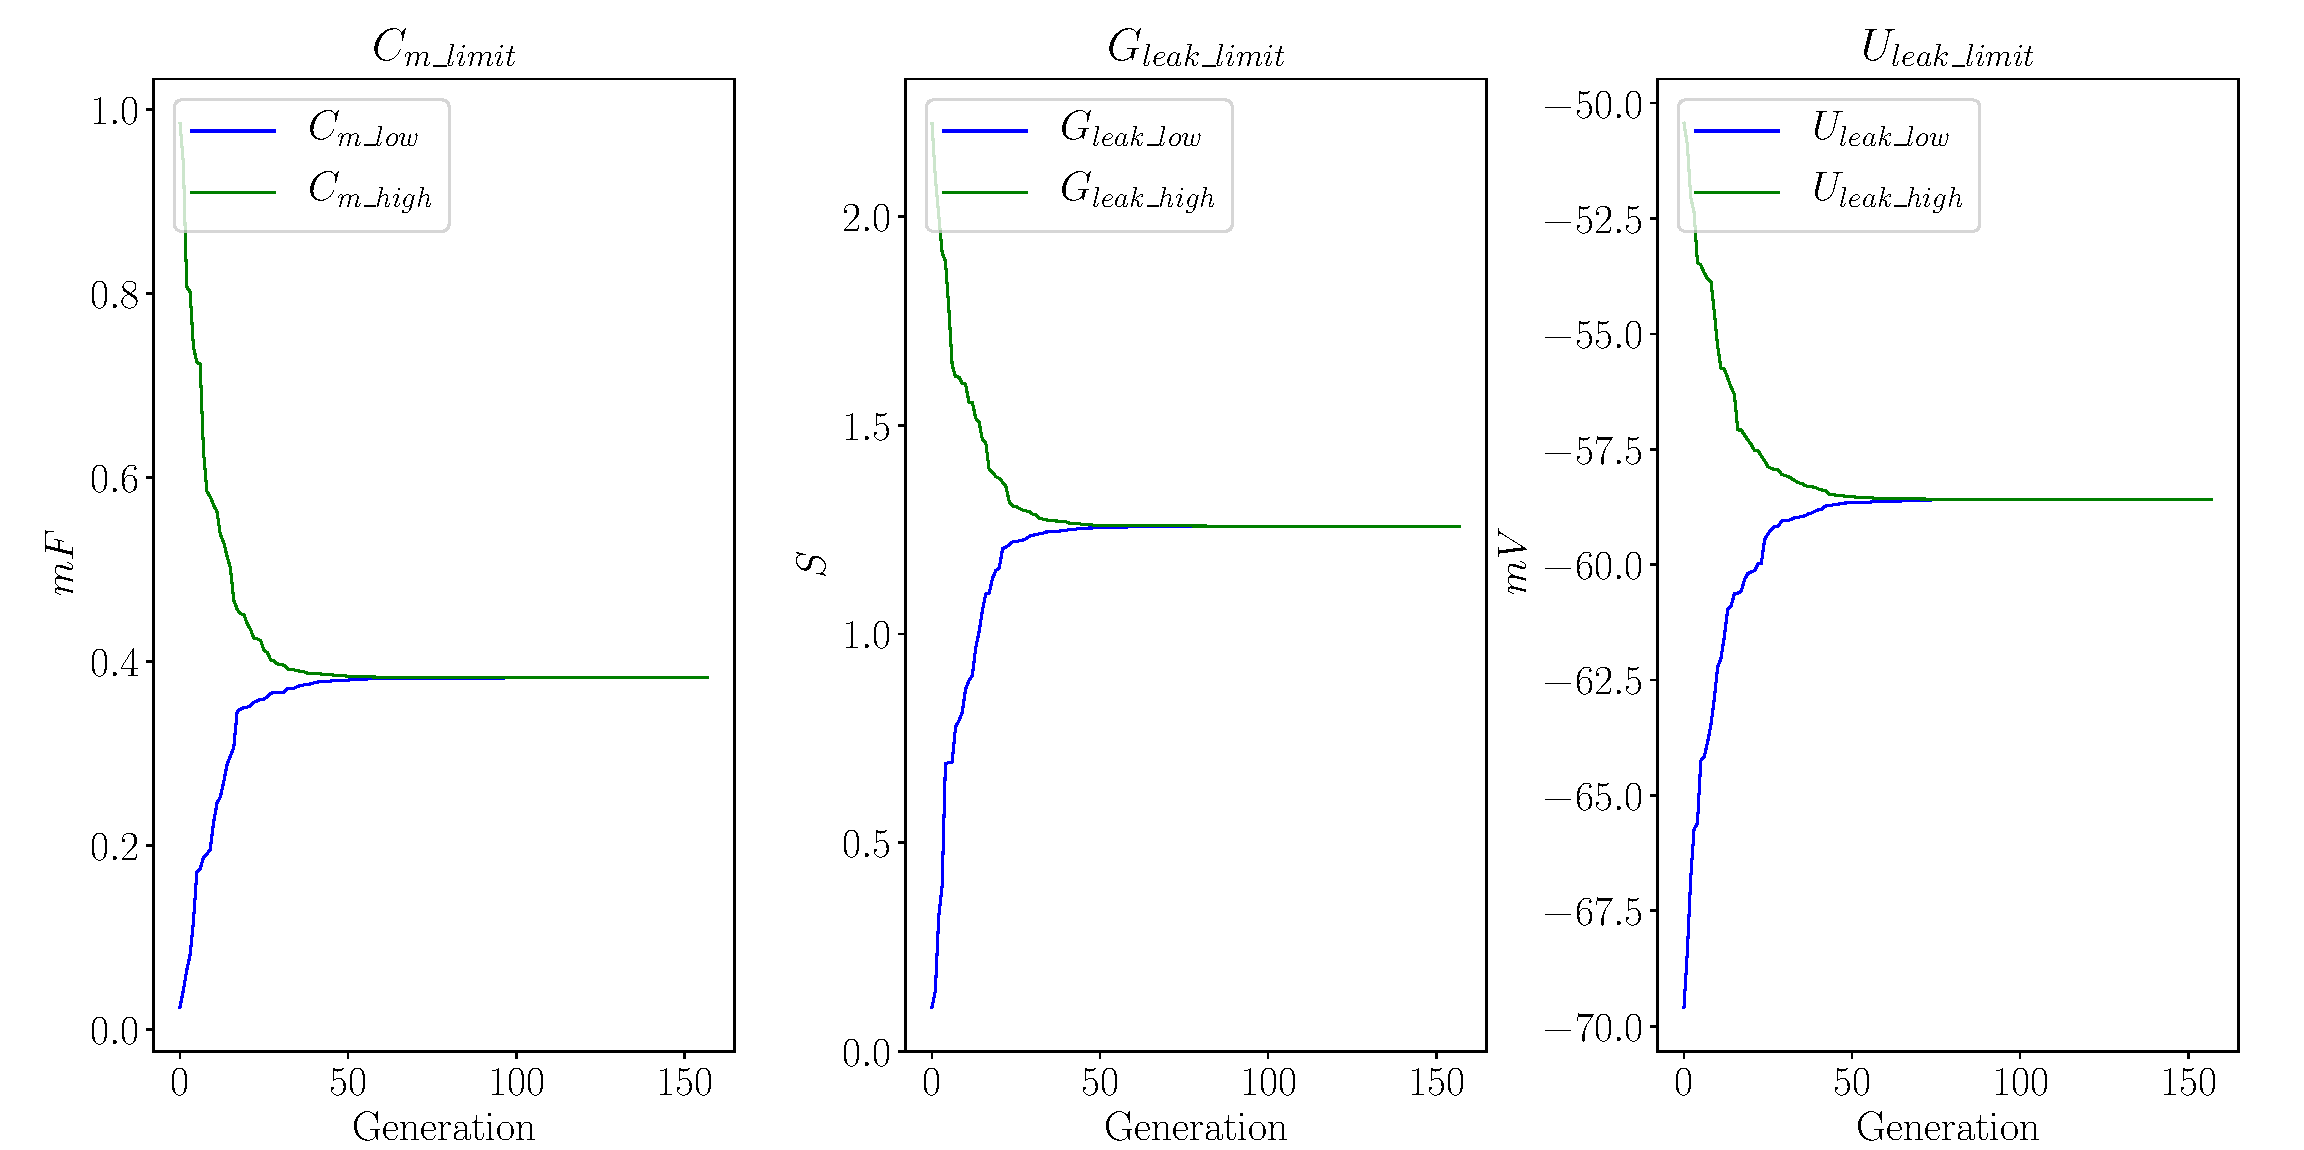
\includegraphics[width=13cm]{figures/chap_implement/ga_neuron.pdf}
			\caption{Plot der Gleichverteilungsgrenzen der Nervenzellen}
			\label{fig:ga_1}
		\end{figure}
		\begin{figure}[H] %[!t] ...
			\centering
			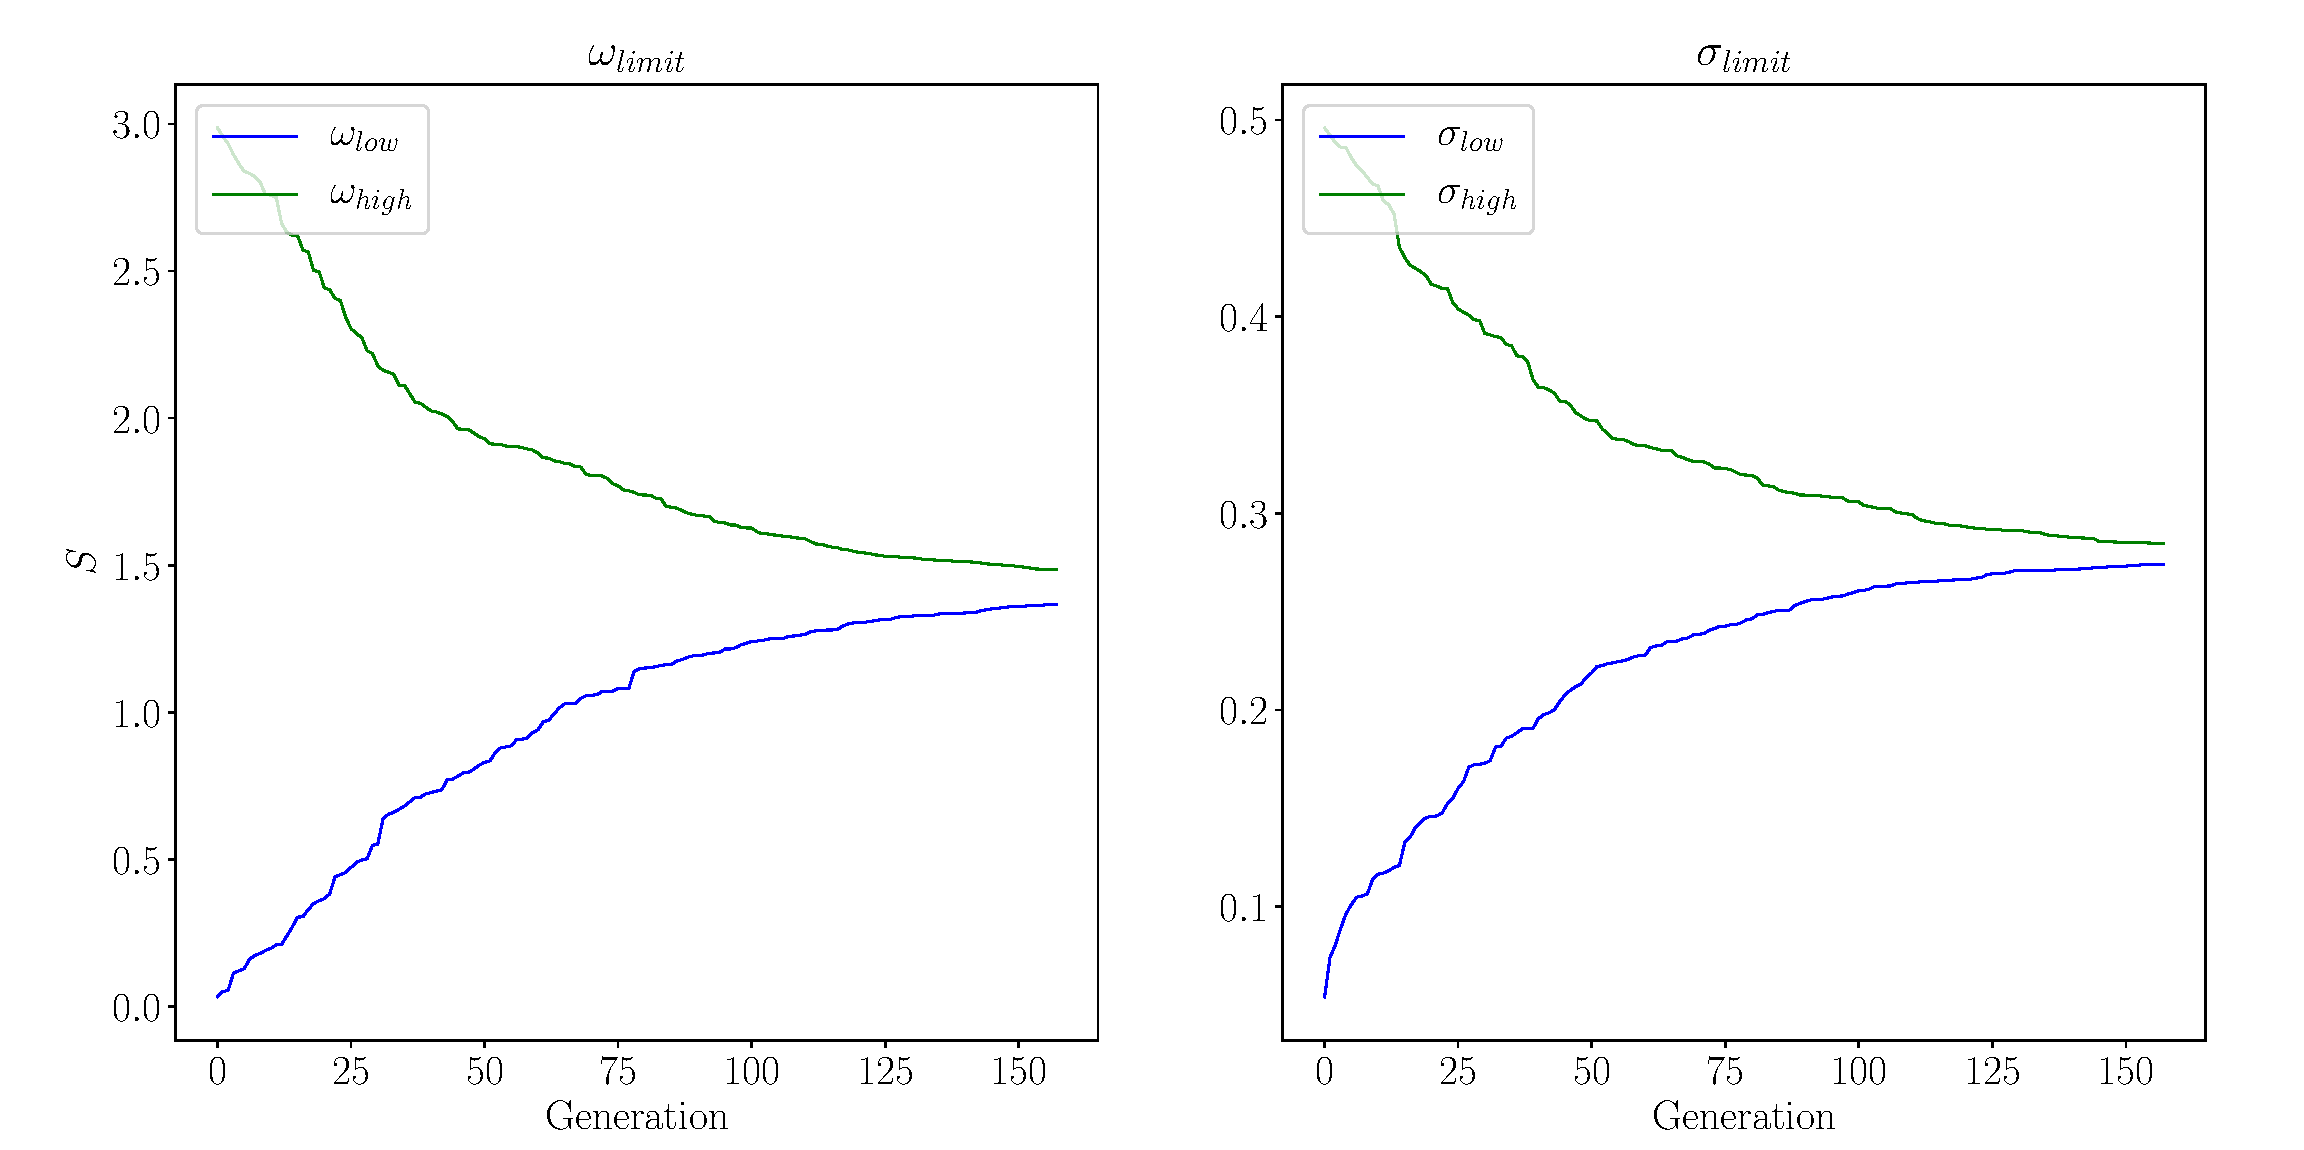
\includegraphics[width=13cm]{figures/chap_implement/ga_synapse.pdf}
			\caption{Plot der Gleichverteilungsgrenzen der Synapsen}
			\label{fig:ga_2}
		\end{figure}
	
	\subsection{Optimierungsalgorithmus Weights}
		Als erstes Optimierungsverfahren nach erfolgreicher Simulation der Parameter des neuronalen Netzes wird nun der Algorithmus Weights eingesetzt. Dieser lässt die bereits simulierten Parameter importieren und gewichtet jede Synapse mit einem Faktor $g\in[0,1]$. Durch einfache Simulationen mit willkürlichen Gewichten wird schnell festgestellt, welche Synapsen bei einem Simulationslauf mit hohem Reward eine große Gewichtung erhalten und welche Synapsen nicht förderlich für das Ergebnis sind. Durch diese Simulation war es möglich, das in Kap. \ref{chap:neuro} vorgestellte symmetrische Neuronale Netz (Abb. \ref{fig:nn_new}) zu entwickeln. Die dort gezeigten Synapsen erfahren eine relevante Gewichtung und sind somit wichtig für den Erfolg des neuronalen Netzes.\\
		Der Gewichtungsalgorithmus ist rechenintensiver als RandomSearch, da insgesamt 16 Synapsen bzw. Gap-Junctions pro Episode mit zufällig gewählten Gewichten versehen werden, um den Reward zu steigern. Jedoch wird ein im Schnitt um das Dreifache höherer Reward verzeichnet bei gleichbleibenden Parametern, was eine sehr gute Optimierung darstellt.\\
		Aufgerufen wird dieser Algorithmus analog zu RandomSearch aus der \texttt{main.py}-Datei. Als Input werden die bereits errechneten optimalen Parameter der jeweiligen Nervenzellen und Synapsen sowie die maximale Simulationszeit eingegeben. Ebenfalls gleich dem Algorithmus RandomSearch produziert Weights einen Dump mit den errechneten Gewichten der Synapsen und Gap-Junctions sowie eine Informationsdatei im \texttt{.txt}-Format, welche weitere Zugehörigkeitsinformationen sowie die Anzahl an Simulationen und die Dauer enthält.
		
	\section{Simulation in der Google Cloud Platform\textsuperscript{\textregistered}}
	Wie bereits in diesem Abschnitt mehrfach erwähnt, sind die implementierten Suchalgorithmen RandomSearch und Weights äußerst rechenintensiv. Beide Skripte erfordern das zufällige Generieren einer hohen Anzahl an Parametern sowie die Anwendung dieser Parameter auf das gegebene Problem durch numerische Lösungsansätze für Differenzialgleichungen (siehe Sektion \ref{sec:lif_imp}). Es müssen Parameter zwischengespeichert und Dumps auf Festplatten geschrieben werden.\\
	Um eine erfolgreiche Simulation des inversen Pendels zu erhalten, muss ein Parametersatz mit hohem Reward gefunden werden, welcher die korrekte Funktionsweise des neuronalen Netzes gewährleistet. Bei dem in Abb. \ref{fig:nn_new} gezeigten neuronalen Netz werden die Parameter $C_m, G_{Leak}, U_{Leak}, \sigma, w, \hat{w}$ für Synapsen, Gap-Junctions und Nervenzellen simuliert.
	\begin{center}
		\begin{tabular}{c@{\hskip 0.5cm}c@{\hskip 0.5cm}c@{\hskip 0.5cm}}    \toprule
			\setlength{\tabcolsep}{50pt}
			\renewcommand{\arraystretch}{1.5}
			\emph{Parameter}	& \emph{Kategorie}  & \emph{Anzahl} \\\midrule
			$C_m$				& Nervenzelle		& 4				\\ 
			$G_{Leak}$	 		& Nervenzelle		& 4				\\
			$U_{Leak}$	 		& Nervenzelle		& 4				\\
			$\sigma$			& Synapse			& 16			\\
			$w$					& Synapse			& 16			\\ 
			$\hat{w}$			& Synapse			& 2				\\\bottomrule
			Gesamt:				&					& \textbf{46}	\\
			\hline
		\end{tabular}
	\end{center}
	Somit werden in jedem Simulationslauf zuerst 46 Parameter in gegebenen Grenzen durch eine Gleichverteilung erzeugt und anschließend durch das \texttt{compute}-Modul (siehe Sektion\ref{sec:lif_imp}) die benötigten Synapsenströme und Membranpotentiale errechnet.\\
	Das Modul Weights erzeugt, analog zu RandomSearch, zuerst für jede Synapse und Gap-Junction ein gleich-verteiltes, zufälliges Gewicht $g\in[0,1]$.
	\begin{center}
		\begin{tabular}{c@{\hskip 0.5cm}c@{\hskip 0.5cm}c@{\hskip 0.5cm}}    \toprule
			\setlength{\tabcolsep}{50pt}
			\renewcommand{\arraystretch}{1.5}
			\emph{Parameter}	& \emph{Kategorie}  & \emph{Anzahl} \\\midrule
			$g$					& Synapse			& 18			\\\bottomrule
			Gesamt:				&					& \textbf{18}	\\
			\hline
		\end{tabular}
	\end{center}
	Somit werden insgesamt 18 Gewichte pro Episode erzeugt und auf das Modell angewendet. Zur Berechnung der erforderlichen Ströme und Potenziale wird das \texttt{compute}-Modul um die Funktion der Gewichtung erweitert.\\
	Ein solches Simulationsvorhaben wird üblicherweise nicht mehr auf Heimrechnern ausgeführt, sondern findet den Weg in die Cloud. Gerade in den letzten Jahren haben Cloud-Computing-Firmen wie Amazon mit AWS\footnote{https://aws.amazon.com/de/}, Microsoft mit der Azure Cloud\footnote{https://azure.microsoft.com/de-de/} und Google mit der Google Cloud Platform (GCP)\footnote{https://cloud.google.com/} an großer Aufmerksamkeit gewonnen. Die einfache Handhabung und Kontrolle über eigene virtuelle Instanzen von ganzen Betriebssystemen erlaubt eine zuverlässige und effiziente Simulation von Parametern. In dieser Angelegenheit wurde sich für die Google Cloud Plattform entschieden, da diese ein sehr gutes User Inferface hat und kostengünstige, virtuelle Maschinen anbietet. Gemietet wurde ein Server mit dem Standort Frankfurt, welcher über vier virtuelle Intel XEON\textsuperscript{\textregistered} Prozessoren sowie 12GB DDR4 Arbeitsspeicher verfügt. Dies erlaubt eine schnelle Simulation von vier Instanzen zur gleichen Zeit sowie den Vorteil, das Langzeitsimulationen von 12 Stunden oder mehr im Hintergrund oder über Nacht erfolgen können.\\
	Auf der virtuellen Instanz wurde ein Linux Ubuntu 18.04 LTS installiert und bereitgestellt. Im nächsten Schritt wird die vorbereitete GitHub Repository auf das System geklont und die benötigten Abhängigkeiten (siehe Anhang \ref{app:datenblatt}) installiert. Durch einen Cronjob werden Skripte ausgeführt und mit \texttt{crontab -e} die Simulation zu einer festen Uhrzeit gestartet. Die übliche Simulationszeit beträgt jeweils 12 Stunden.\\
	\begin{minipage}[c]{0.5\textwidth}
		\begin{figure}[H] %[!t] ...
			\centering
			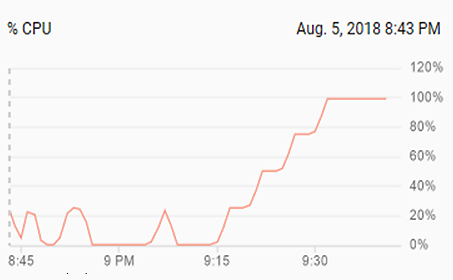
\includegraphics[width=7cm]{figures/chap_implement/GCP.png}
			\caption{Systemauslastung der virtuellen Instanz - GCP Dashboard}
			\label{fig:gcp_1}
		\end{figure}
	\end{minipage}
	\begin{minipage}[c]{0.5\textwidth}
		\begin{figure}[H] %[!t] ...
			\centering
			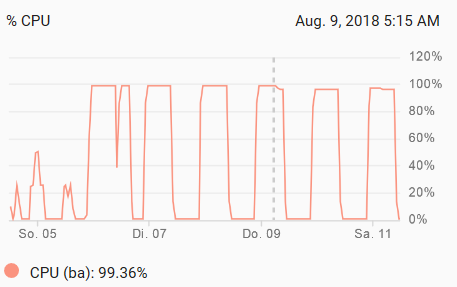
\includegraphics[width=7cm]{figures/chap_implement/GCP_2.png}
			\caption{Systemauslastung der virtuellen Instanz im Dauerbetrieb (Cronjob)}
			\label{fig:gcp_2}
		\end{figure}
	\end{minipage}\vspace{0.5cm}
	Wie in Abb. \ref{fig:gcp_1} und \ref{fig:gcp_2} zu sehen, werden die Suchalgorithmen nacheinander durch den Cronjob ausgeführt, da pro Suchlauf nur ein Prozessorkern in Anspruch genommen werden kann. Der virtuelle Prozessor erreicht somit bei vier gleichzeitigen Simulationsläufen eine Auslastung von $100\%$.\\
	Die Ergebnisse der Suchläufe werden in Form von Parameter- und Weight-Dumps via eines Apache Webservers bereitgestellt und können problemlos auf dem Heimrechner visualisiert werden. Durch das gewählte Dateiformat der Dumps in HDF5 \cite{hdf5} sind die Dateien Plattformunabhängig und äußerst performant lesbar. Diese Methode funktioniert darüber hinaus auch Versionsübergreifend. Eine Simulation kann Dumps mit Python 2.7 erstellen, welche durch einen Heimrechner mit Python 3.x visualisiert werden können.

% ***
\section{Simulationsumgebung: OpenAI Gym}
\label{sec:imp_sim}
% ***
	Um die Performance eigener neuronaler Netze und Algorithmen zu messen, wurden in den letzten Jahren eine ganze Reihe an Simulationen und Spielen entwickelt. Ziel dieser Simulationsumgebungen ist es, die Entscheidung des Agenten in gewissen Situationen zu testen und den Lernerfolg darzustellen. Darüber hinaus wird das Verständnis für neuronale Netze durch das Anwenden auf Spiele und Experimente vertieft.\\
	Eine sehr bekannte Open Source Bibliothek an Simulatoren und Spielen ist Gym von OpenAI\footnote{https://openai.com/}. OpenAI ist eine Non-Profit Organisation mit dem Ziel, den Forschungsbereich der künstlichen Intelligenz voran zu treiben und ein besseres Verständnis für die Vorgänge in neuronalen Netzen zu schaffen. Die Bibliothek Gym enthält verschiedene Umgebungen:
	\begin{itemize}
		\item Algorithmen:
		\subitem Einfache Aktionen wie Copy-Paste, Addition und Subtraktion sowie logische Gatter
		\item Atari
		\subitem Sammlung an klassischen Atari Spielen wie Breakout, Pacman und Space Invaders
		\item Classic Control
		\subitem Simulationsumgebungen wie das inverse Pendel oder das Mountain Car
		\item Robotics
		\subitem Komplexe Simulationen von Roboterarmen oder -händen
	\end{itemize}
	In dieser Arbeit wird die Umgebung \texttt{CartPole\_v0} (Abb. \ref{fig:imp_cartpole}) gewählt. Diese besteht aus einem einfachen inversen Pendel, welches sich auf einer zweidimensionalen Bahn frei bewegen kann.
	\begin{figure}[H] %[!t] ...
		\centering
		\def\svgwidth{12cm}
		\input{figures/chap_implement/cartpole.pdf_tex}
		\caption{Simulationsumgebung \texttt{CartPole\_v0}.}
		\label{fig:imp_cartpole}
	\end{figure}
	Die Handhabung dieser Simulationsumgebung ist dank einer großen Community und guten Dokumentationen sehr einfach. Initialisiert wird die Umgebung, indem die Bibliothek \texttt{gym} in das Python-Skript importiert und die gewählte Umgebung als \glqq Environment\grqq{}festgelegt wird. Pro Simulationsschritt kann eine Aktion $a = \{0,1\}$ getätigt werden.
	\begin{align*}
		0 :& \text{ Schritt nach Links}\\
		1 :& \text{ Schritt nach Rechts}
	\end{align*}
	Das bereits vorgestellte neuronale Netz (Abb: \ref{fig:nn_new}) verfügt über zwei Motor-Neuronen, welche als Eingang der Simulation genutzt werden können. Interne Nervenzellen \textit{AVA} und \textit{AVB} sind durch eine direkte Synapse mit den genannten Motor-Neuronen verbunden und verursachen im Falle eines Fire-Events die Bewegung des Wagens um einen Schritt nach links bzw. rechts. Pro Simulationsschritt erfolgt je nach Observation immer ein Fire-Event, sodass das Pendel zu jeder Zeit eine berechnete Aktion erhält.
	\begin{figure}[H] %[!t] ...
		\centering
		\def\svgwidth{12cm}
		\input{figures/chap_implement/cartpole_FWD_REV.pdf_tex}
		\caption{Simulationsumgebung \texttt{CartPole\_v0} mit Aktionen \textit{FWD} und \textit{REV}.}
		\label{fig:imp_cartpole_FWD_REV}
	\end{figure}
	Pro Simulationsschritt wird ein Observationsvektor ausgegeben. Dieser enthält die folgenden Parameter:
	\begin{align}
		\boldsymbol{o} &= \begin{pmatrix}C_{Position} & C_{Velocity} & P_{Angle} & P_{Velocity}\end{pmatrix}\text{.}
	\end{align}
	\begin{center}
		\begin{tabular}{c@{\hskip 0.5cm}c@{\hskip 0.5cm}r@{\hskip 0.5cm}}    \toprule
			\setlength{\tabcolsep}{50pt}
			\renewcommand{\arraystretch}{1.5}
			\emph{Parameter}	& \emph{Beschreibung}  				& \emph{Grenzen} 			\\\midrule
			$C_{Position}$		& Position des Carts				& $[-2.4, 2.4]$				\\
			$C_{Velocity}$		& Geschwindigkeit des Carts			& $(-\infty, \infty)$		\\
			$P_{Angle}$			& Winkel des Pendels				& $[-41,8^{\circ}, 41,8^{\circ}]$	\\
			$P_{Velocity}$		& Winkelgeschwindigkeit des Pendels	& $(-\infty, \infty)$		\\\bottomrule
			\hline
		\end{tabular}
	\end{center}
	\begin{figure}[!h] %[!t] ...
		\centering
		\def\svgwidth{12cm}
		\input{figures/chap_implement/cartpole_observation.pdf_tex}
		\caption{Simulationsumgebung \texttt{CartPole\_v0} mit Observationsgrößen.}
		\label{fig:imp_cartpole_observation}
	\end{figure}
	Die Informationen aus dem Observationsvektor $\boldsymbol{o}$ werden entsprechend interpretiert und den Sensor-Neuronen zugeführt. Wie bereits in Sektion \ref{sec:neuro_netz} beschrieben, ist der Winkel des Pendels $\varphi$ als primäre Größe den Sensor-Neuronen \textit{PLM} und \textit{AVM} zuzuführen. Als sekundäre Größe kann die Winkelgeschwindigkeit $\dot{\varphi}$ oder die Position des Carts $x$ den Sensor-Neuronen \textit{ALM} und \textit{PVD} zugeführt werden. Die Wahl der geeigneten sekundären Observationsgröße ist dem neuronalen Netz zuzuschreiben. Durch die inhibitorische Beeinflussung durch Sensor-Neuronen \textit{ALM} und \textit{PVD} entsteht ein dämpfendes Signal, welches dafür sorgt, dass bei zu hoher Winkelgeschwindigkeit oder Cartposition die Kompensation durch Bewegung des Carts nicht übersteuert. Ergebnisse durch Wahl der geeigneten sekundären Sensorgröße werden in Kapitel \ref{chap:erg} erläutert.

% ***
\section{Visualisierung und Auswertung}
\label{sec:imp_vis}
% ***
	Wie bereits in Sektion \ref{sec:imp_sim} näher beschrieben, liefert die Simulationsumgebung \texttt{CartPole\_v0} eine sehr gute Echtzeitvisualisierung des inversen Pendels als Animation. Diese wird durch das Speichern eines errechneten RGB-Tensors jedes Simulationsschrittes und anschließenden Animieren der Informationen erreicht. Weiterhin soll das Programm jedoch in der Lage sein, wichtige Parameter der Simulation über die Simulationszeit darzustellen, um ggf. Probleme zu erkennen und Aktionen zu verstehen. Um Plots aus Arrays zu erstellen, wird die Python-Bibliothek \texttt{matplotlib} \cite{Hunter2007} genutzt. Durch die einfache Bedienung und den enormen Umfang an Werkzeugen ist diese Bibliothek sehr beliebt in der Visualisierung von Daten und Parametern.\\
	Der generelle Ablauf des Programms sieht im ersten Schritt die Simulation von Parametern und Gewichten vor. Dies erfordert keine Visualisierung der Vorgänge, da die Performance erheblich beeinträchtigt werden würde. Daher wurde das Modul \texttt{visiualize.py} geschrieben, um gefundene Parameter und Gewichte mühelos simulieren zu können. Für den Aufruf werden die entsprechenden Parameter- und Gewichte-Dumps übergeben sowie die gewünschte Simulationszeit (bspw. 5 Sekunden). Die Simulation wird analog in den Suchalgorithmen jedoch mit festen Parametern ausgeführt. Gewünschte Größen werden pro Simulationsschritt gespeichert und letztlich grafisch dargestellt. Besonders die Übersicht über die Membranpotentiale einzelner Nervenzellen bietet einen sehr guten Überblick über die Vorgänge im neuronalen Netz und die Reaktion auf gegebene Sensor-Daten.
	\begin{figure}[H] %[!t] ...
		\centering
		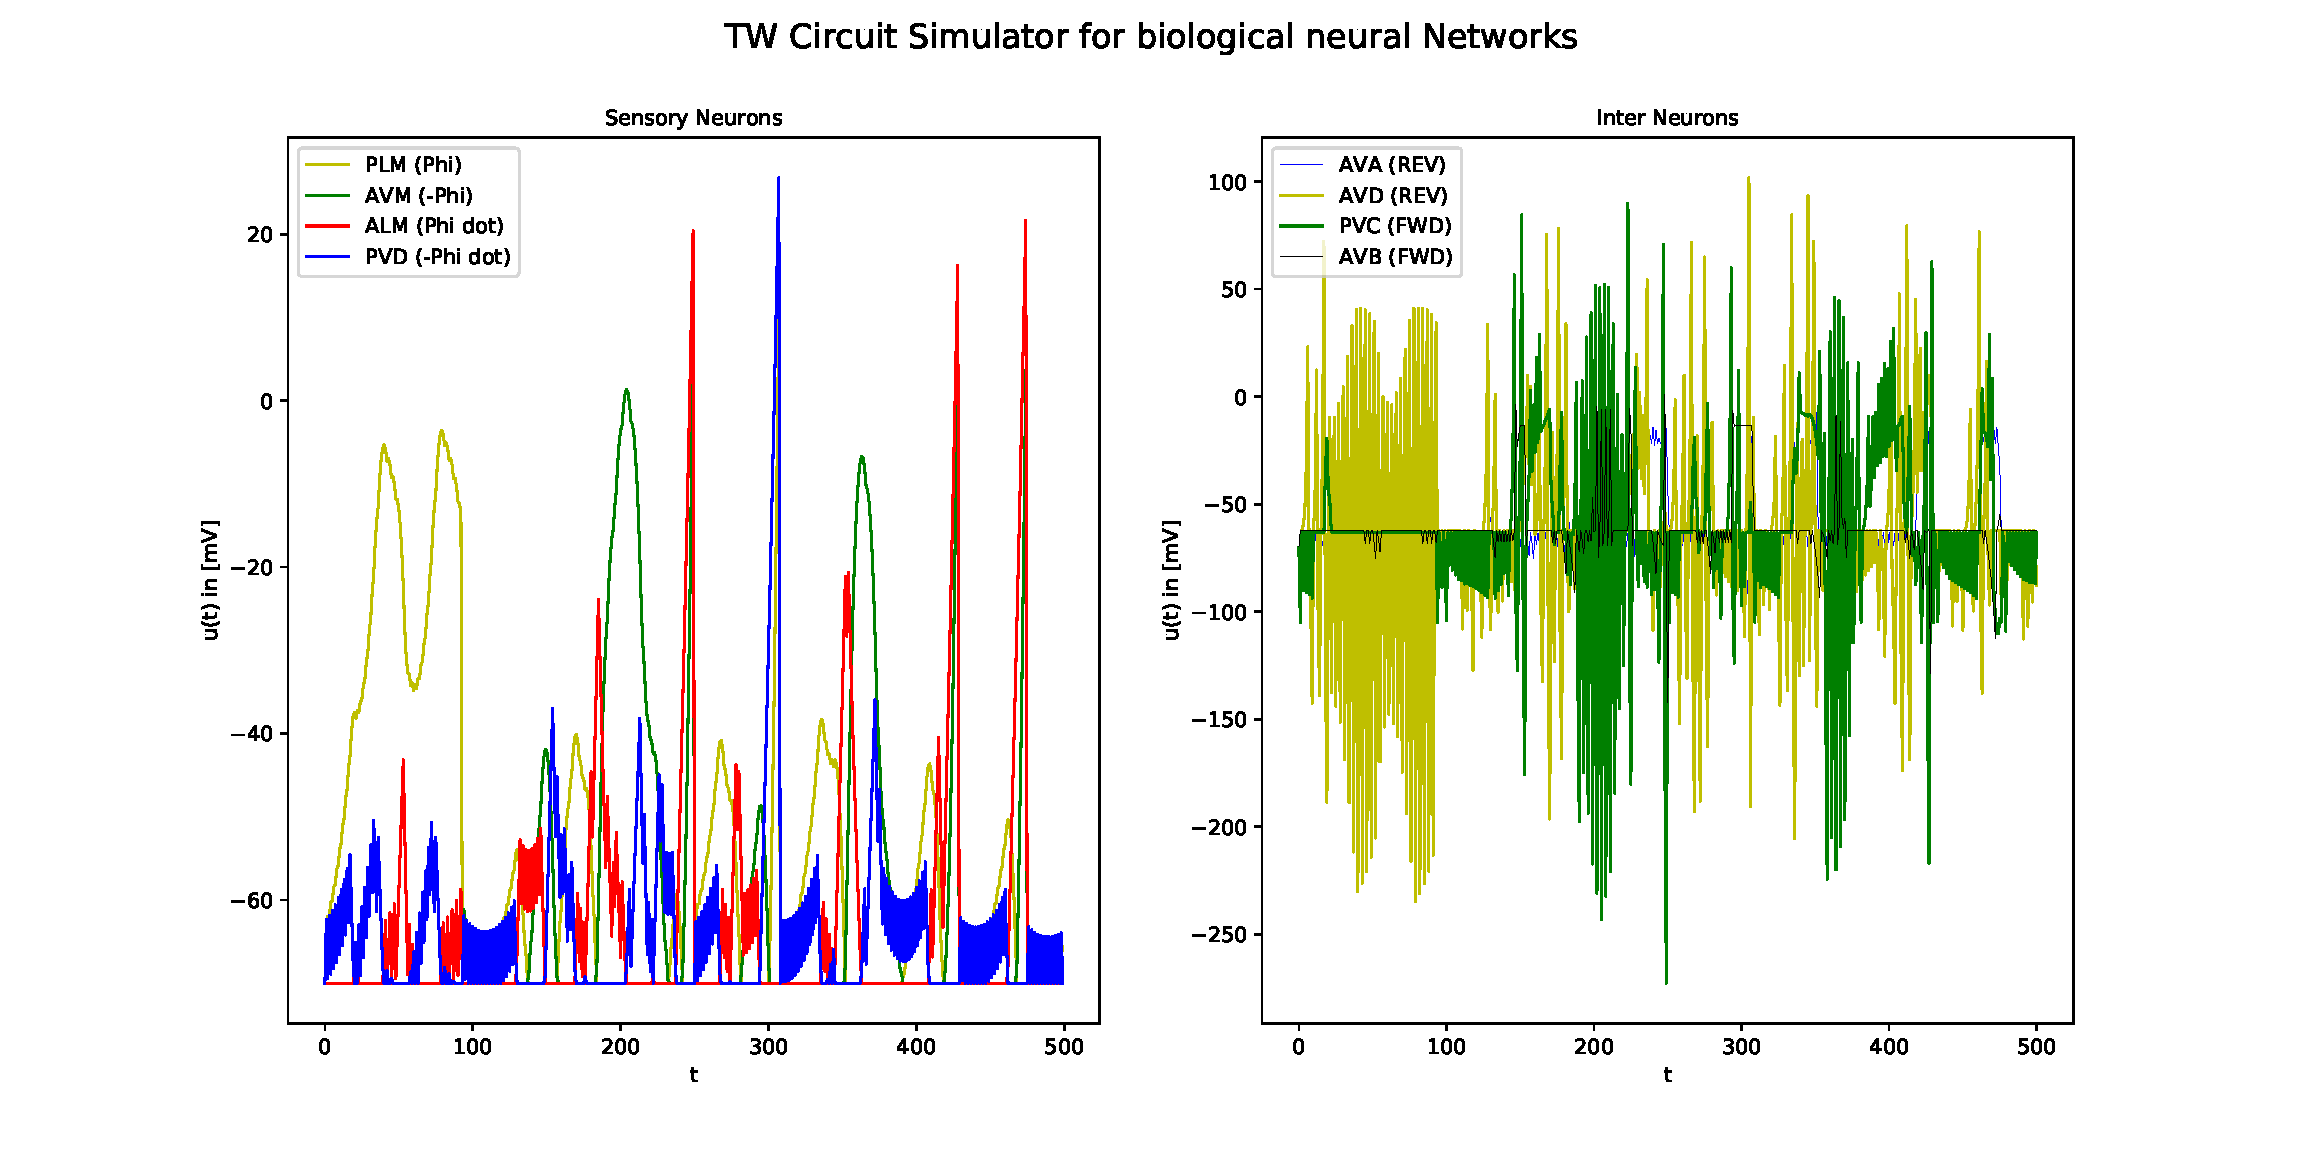
\includegraphics[width=16cm]{figures/chap_implement/plot_membranpot.pdf}
		\caption{Plot der Membranpotentiale von Inter- und Sensorneuronen}
		\label{fig:plot_membr}
	\end{figure}
	Weiterhin wird standardmäßig neben den Membranpotentialen auch der anliegende Synapsenstrom an jeder Nervenzelle geplottet. Diese Veranschaulichung gibt Aufschluss über die gewählten Parameter und das Feuerverhalten im internen neuronalen Netzwerk.
	\begin{figure}[H] %[!t] ...
		\centering
		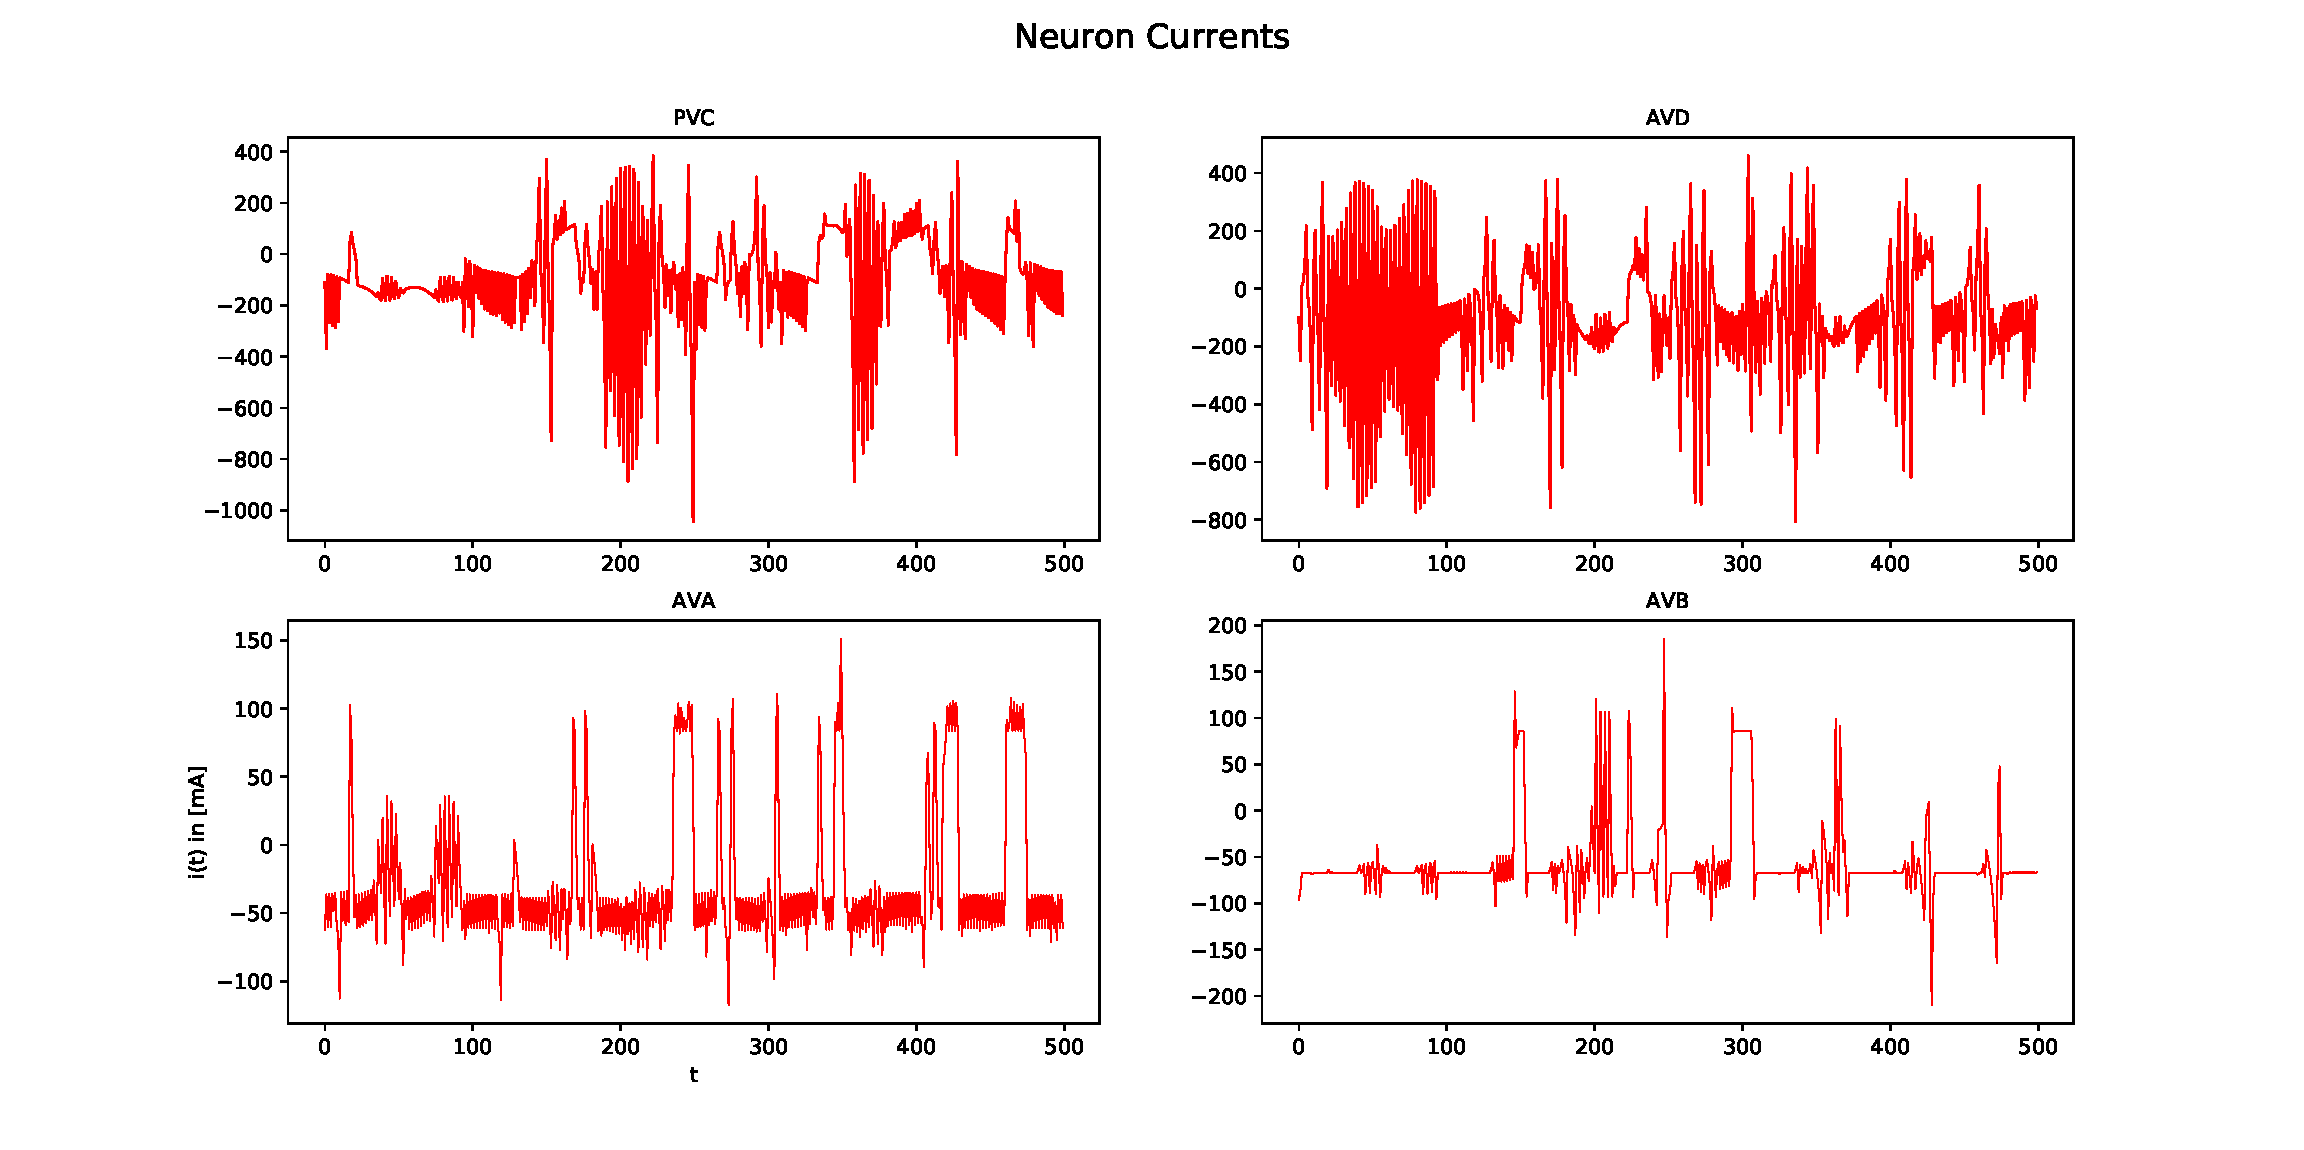
\includegraphics[width=16cm]{figures/chap_implement/plot_synstrom.pdf}
		\caption{Plot der anliegenden Ströme aus Stimulus, Synapsen und Gap-Junctions}
		\label{fig:plot_synstrom}
	\end{figure}

% ***
\section{Sonstige Implementierung}
\label{sec:imp_sonst}
% ***
	Neben den prominenten Modulen wurden im Laufe der Zeit mehrere hilfreiche Nebenmodule und Funktionen implementiert sowie notwendige Pakete genutzt.
	\subsection{Zentraler Ort für Parameter}
		Um einen zentralen Ort für verschiedene Größen und Parameter zu schaffen, wurde das Modul \texttt{parameters.py} erstellt. Dieses Modul wird im gesamten Programm eingebunden und dient als globale Informationsbasis. Nur wenige Größen können verändert werden wie bspw. die Transitionsmatrizen des neuronalen Netzes oder manche Parameter zur Berechnung von Synapsenströmen und Membranpotentialen. Alle weiteren Daten werden automatisch berechnet und im Laufe der Simulation bereitgestellt.
	\subsection{Speicherung von Daten}
		Ein Problem, welches über die Implementierung aufkam, war die Speicherung von Dateien in s.g. Dump-Files. Nach einer erfolgreichen Simulation von Parametern soll der beste Parametersatz zur weiteren Analyse gespeichert werden. Dazu liefert Python die Bibliothek \texttt{Pickle}, welche verschiedene Datentypen seriell in ein kompaktes Binärformat konvertiert und in der \texttt{.p} Dateiendung speichert. Dieser Vorgang ist jedoch besonders mit Python 2.7 verhältnismäßig langsam und beeinträchtigt die Performance der Simulation. Darüber hinaus besteht eine Inkompatibilität des Dateiformats zum einen zwischen verschiedenen Python-Versionen, zum anderen unter unterschiedlichen Betriebssystemen.\\
		Eine elegantere Möglichkeit bietet die Open Source Bibliothek \texttt{hickle}. Sie wird ähnlich wie \texttt{pickle} importiert und speichert die gewählten Parameter in einer \texttt{.hkl}-Datei. Die Daten werden anders als bei Pickle im s.g. HDF5 (Hierarchical Data Format 5) \cite{hdf5} gespeichert. Dies ist zum einen performanter, sorgt zum anderen für eine erheblich größere Kompatibilität unter Python-Versionen und Betriebssystemen.
	\subsection{Dateiinspektion}
		Besonders nach den ersten Simulationen ist die Inspektion der errechneten Parameter und Gewichte von äußerster Wichtigkeit. Hohe Rewards bedeuten nicht direkt, dass das neuronale Netz in jeder Situation richtig oder gut performt. Beispielsweise kann ein sehr guter Reward in der Bewegung des Pendels in Vorwärtsrichtung erreicht werden, obwohl die Parameter der Rückwärtsbewegung nicht sehr gut ausgereift sind. Daher wird ein Modul zur detaillierten Inspizierung der Dump-Dateien \texttt{inspect.py} geschrieben. Bei Aufruf einer Funktion dieses Moduls muss jeweils der Pfad der Dump-Datei übergeben werden. Die Datei wird geöffnet und die Parameter den entsprechenden Größen zugewiesen. Danach kann ein Konsolen-Output erfolgen oder ein Plot der gespeicherten Daten erzeugt werden.


%%% Local Variables: 
%%% mode: latex
%%% TeX-master: "main"
%%% End: 

%
% ****
\chapter{Performance \& Auswertung}
\label{chap:erg}
% ****
%
	Dieses Kapitel dient der Auswertung von Versuchsergebnissen und dem Vergleich der verschiedenen Suchalgorithmen. Ausgangspunkt und somit Vergleichskriterium sind Simulationsgrößen des inversen Pendels \texttt{CartPole\_v0} des Frameworks OpenAI \texttt{Gym}.	Es wurde zuerst eine Berechnungsgrundlage eines neuronalen Netzes nach \textit{C. Elegans} \cite{CElegans} geschaffen und implementiert. Dazu wurden verschiedene numerische Lösungsverfahren von Differentialgleichungen verglichen und umgesetzt \cite{NonlinearDynamics}. Letztlich wird ein universeller Simulator geschaffen, welcher Informationen über die Nervenzellen und Synapsen erhält und entsprechend in der Lage ist, das Netz zu simulieren und Feuer-Events auszugeben. Um die Performance des neuronalen Netzes durch den Simulator zu messen, wird eine Simulationsumgebung eingebunden und ein Lern-Algorithmus implementiert. Im Folgenden wird sich auf die \textit{Reinforcement Learning} Methode Random-Search konzentriert, die Methode der genetischen Algorithmen untersucht und auf die Optimierungsmethode durch Gewichten der entsprechenden Synapsen eingegangen.

% ***
\section{Performance implementierter Algorithmen}
\label{sec:erg_performance}
% ***
	Die Schnelligkeit der Ausführung von Algorithmen und ganzen Skripten ist in dieser Anwendung von großer Relevanz. Da der Simulator von Grund auf darauf ausgerichtet worden ist, später rechenintensive Simulationen von Parametern zu durchlaufen, wird bereits in der Auswahl der zusätzlich genutzten Pakete darauf geachtet, diese performant und ressourceneffizient zu implementieren.
	
	Angefangen bei den Berechnungsmodulen in der Datei \texttt{lif.py} wird für komplexere mathematische Operationen die Erweiterung \texttt{NumPy} \cite{NumPy} aus dem bekannten Python-Paket \texttt{SciPy} \cite{NumPy} genutzt. Außerdem werden Schleifen und If-Abfragen ohne Redundanzen und unnötige Befehle implementiert, um in der höheren Abstraktionsebene einen einwandfreien Aufruf zu garantieren. Nach erfolgreichen Tests der implementierten Funktionen ist das Framework für den Simulator erstellt worden. Genutzte Pakete wie \texttt{matplotlib} \cite{Hunter2007} oder \texttt{Hickle} \cite{hdf5} sind ebenfalls für ihre Schnelligkeit und einfache Handhabung ausgewählt worden. Des Weiteren können hier die bereits implementierten Funktionen zur Berechnung von Synapsenströmen und Membranpotentialen einfach importiert werden.
	
	Letztendlich ist die Ausführung der Suchalgorithmen Random-Search und Genetic Algorithm sowie die Optimierung durch den Algorithmus Weights ausschlaggebend. Diese Algorithmen wurden im Laufe der Implementierung immer wieder optimiert und verbessert, sodass eine zuverlässige Simulation mit effizienten Laufzeiten möglich wird. Bei festen Simulationszeiten werden auf der bereits vorgestellten virtuellen Instanz folgende Ergebnisse erzielt (stichprobenartig aufgelistet):
	\begin{table}[H]
		\centering
		\resizebox{0.6\columnwidth}{!}{%
		\begin{tabular}{c@{\hskip 0.5cm}c@{\hskip 0.5cm}c@{\hskip 0.5cm}c}    \toprule
			\setlength{\tabcolsep}{50pt}
			\renewcommand{\arraystretch}{1.5}
			\emph{Zeitstempel}	& \emph{Belohnung} 	& \emph{Laufzeit}	& \emph{Anz. Simulationen} 	\\\midrule
			20180815\_10-40-23  & 26				& 2 Std.			& $39.006$					\\ 
			20180816\_01-50-01	& 123				& 12 Std.			& $10.509.904$				\\
			20180816\_01-52-01	& 185				& 12 Std.			& $10.536.512$				\\
			20180818\_02-48-01	& \textbf{200}		& 12 Std.			& $10.852.326$				\\\bottomrule
			\hline
		\end{tabular}}
	\caption{Parametersuche durch Algorithmus \texttt{Random-Search}.}
	\label{tab:sim_rs}
	\end{table}
	\begin{table}[H]
		\centering
		\resizebox{0.6\columnwidth}{!}{%
		\begin{tabular}{c@{\hskip 0.5cm}c@{\hskip 0.5cm}c@{\hskip 0.5cm}c}    \toprule
			\setlength{\tabcolsep}{50pt}
			\renewcommand{\arraystretch}{1.5}
			\emph{Zeitstempel}	& \emph{Belohnung} 	& \emph{Laufzeit}	& \emph{Anz. Simulationen} 	\\\midrule
			20180815\_11-21-46  & 56				& 1 Std.			& $5.927$					\\ 
			20180816\_13-50-01	& 149				& 12 Std.			& $3.715.008$				\\
			20180816\_13-52-01	& \textbf{200}		& 12 Std.			& $3.686.723$				\\\bottomrule
			\hline
		\end{tabular}}
		\caption{Optimierung durch Algorithmus \texttt{Weights}.}
		\label{tab:sim_weights}
	\end{table}
	Diese Simulationen wurden ausnahmslos auf derselben virtuellen Instanz (parallel) ausgeführt. Die genauen Spezifikationen wurden in Abschnitt \ref{sec:imp_search} bereits detailliert beschrieben. Auffällig ist die unterschiedliche Anzahl an Simulationen bei gleichbleibender Zeit zwischen dem Suchalgorithmus Random-Search und dem Optimierungsalgorithmus Weights. Im Schnitt werden bei der Parametersuche ca. 11 Mio. Simulationen in einem Zeitraum von 12 Stunden erfasst. Die nachgelagerte Optimierung durch den Algorithmus Weights ist jedoch rechenintensiver und erfasst innerhalb 12 Stunden lediglich ca. 3,7 Mio. Simulationen.
	
	Der Suchalgorithmus Genetic Algorithm ist nicht auf lange Simulationszeiten ausgelegt. Durch die zielgerichtete Suche über mehrere Generationen hinweg werden die Grenzen der Gleichverteilung von Parametern aktualisiert und pendeln sich innerhalb weniger Minuten ein (siehe Abbildungen \ref{fig:ga_1} und \ref{fig:ga_2}). Doch wie bereits in Abschnitt \ref{subsec:gen_alg} angedeutet, wird in jedem Simulationslauf lediglich ein lokales Maximum gefunden. Dieses ist nur mit geringer Wahrscheinlichkeit auch das globale Optimum der Simulationsumgebung.
	\begin{table}[H]
		\centering
		\resizebox{0.6\columnwidth}{!}{%
			\begin{tabular}{c@{\hskip 0.5cm}c@{\hskip 0.5cm}c@{\hskip 0.5cm}c}    \toprule
				\setlength{\tabcolsep}{50pt}
				\renewcommand{\arraystretch}{1.5}
				\emph{Zeitstempel}	& \emph{Belohnung} 	& \emph{Laufzeit}	& \emph{Anz. Simulationen} 	\\\midrule
				20180905\_10-12-08  & 11				& 10 Min			& $253.416$					\\ 
				20180905\_10-22-08	& \textbf{200}		& 10 Min			& $276.505$				\\
				20180905\_11-22-08	& 31				& 10 Min			& $295.116$				\\\bottomrule
				\hline
		\end{tabular}}
		\caption{Parametersuche durch Algorithmus \texttt{Genetic\_Algorithm}.}
		\label{tab:sim_gen}
	\end{table}
	Wie der Tabelle \ref{tab:sim_gen} zu entnehmen ist, ergeben Simulationen gleicher Dauer stark divergente Belohnungs-Ergebnisse.
	
	Letztendlich zeigen diese Daten, dass die implementierten Algorithmen in der Lage sind, dauerhafte Simulationen mit guten Ergebnissen zu erzielen. Durch kleinere Verbesserungen und Veränderungen am Code erzielte der Parametersuchlauf mit dem Zeitstempel \texttt{20180817\_01-56-01} das erste Mal eine Belohnung von 200. Dieses Ergebnis beweist die Funktionsweise des Simulators und hält das Pendel in 200 von 200 Simulationsschritten erfolgreich aufrecht. Eine Animation dieser Parameter wird in Appendix \ref{app:parameter} genauer erläutert und veranschaulicht.
	
% ***
\section{Limitationen und Alternativen von Algorithmen}
\label{sec:erg_lim}
% ***
	Die bereits vorgestellten Algorithmen \texttt{Random-Search} als Such- und \texttt{Weights} als Optimierungsalgorithmus führen zwar mit viel Rechenleistung und hohen Simulationszeiten zu guten und verlässlichen Ergebnissen, sind jedoch im Grunde ineffizient. Einzig die Herangehensweise durch genetische Algorithmen ist nicht sehr rechenintensiv, liefert jedoch durch die zielgerichtete Suche meist ein lokales Maximum der Belohnungsfunktion, welches meist eine geringe Belohnung aufweist.\\
	\subsection{Analyse bereits bestehender Algorithmen}
		\texttt{Random-Search} generiert Vektoren mit zufälligen Parametern innerhalb einer gegebenen Gleichverteilung und wendet diese auf die Simulationsumgebung an. Die Belohnung am Ende einer jeden Simulation sagt etwas über die Güte dieser generierten Parameter aus. Ist die Belohnung hoch, so werden die Parameter gespeichert, fällt die Belohnung geringer als die bisher beste Belohnung aus, wird diese Simulation verworfen. So baut sich ein High-Score-System auf und nach Ablauf der Simulationszeit werden die Parameter mit der höchsten erreichten Belohnung gespeichert.	Wie darüber hinaus in Abbildung \ref{fig:uml_rs} noch einmal verdeutlicht, werden gute Parameter für stabile Simulationsläufe durch den simplen Input der Belohnung gefunden.
		
		Analog zu \texttt{Random-Search} beginnt der Algorithmus \texttt{Genetic Algorithm} mit zufälligen Parametern in gegebenen Grenzen. Nach einer festen Anzahl an Episoden ist eine Generation vollendet und wird untersucht. Maxima und Minimal der Parameter werden isoliert und als neue Grenzen der Gleichverteilung für zufällige Parameter gesetzt. Ein High-Score-System ermittelt wieder die besten Simulationen und entsprechende Parameter werden gespeichert (siehe Abbildung \ref{fig:uml_ga}).
		
		Nach Anwendung der Parametersuche durch \texttt{Random-Search} oder \texttt{Genetic Algorithm} wird eine Optimierung des neuronalen Netzes durch den Optimierungsalgorithmus \texttt{Weights} durchgeführt. Durch das Einführen von Gewichten für Synapsen und Gap-Junctions, können gewisse Informationsbahnen eingestellt und die Simulation weiter verbessert werden. In Abbildung \ref{fig:uml_weights} wird der gesamte Programmablauf noch einmal verdeutlicht. Gefundene Parameter und Gewichte guter Simulationsläufe werden in Anhang \ref{app:parameter} aufgeführt.
		
		Aufgrund der starken Symmetrie des gegebenen Problems und des neuronalen Netzes ist es darüber hinaus möglich, eine symmetrische Parameter- und Gewichtsgenerierung zu implementieren. Anstatt der gesamten 46 Parameter für Nervenzellen Synapsen und Gap-Junctions, werden jeweils nur die Hälfte der benötigten Parameter generiert und anschließend dupliziert. Dies sorgt für eine symmetrische Verteilung von zufällig generierten Parametern und einer noch effizienteren Simulation.
	\subsection{Alternative Such- und Optimierungsalgorithmen}
		Wie bereits in Abschnitt \ref{sec:rl_alt} vorgestellt, existieren bereits viele gute Algorithmen zur Parametersuche und -optimierung von künstlich erzeugten oder gegebenen neuronalen Netzen. Doch die Implementierung dieser Algorithmen, besonders auf die hohe Anzahl an zu variierenden Parametern, stellt eine erweiterte Anforderung dar.
		
		Der in Abschnitt \ref{subsec:rl_qlearning} zuerst vorgestellte Algorithmus des Q-Learning ist speziell für die neuen Praktiken der künstlich erschaffenen neuronalen Netze entwickelt worden. Hier wird auf die Gewichtung vieler einfacher Verbindungen zwischen Neuronen unterschiedlicher Ebenen fokussiert. Die Grundlagen könnten auf einfache Parameteroptimierungen angewendet werden, jedoch ist dieser Aspekt größtenteils unerforscht.
		
		Die Methode, durch \textit{Gradient Policies} eine Parameteroptimierung durchzuführen, ist durchaus möglich und kann zu effizienteren Simulationslaufzeiten führen. Problematisch ist aber die Tatsache, dass sich durch die Anzahl an zu simulierenden Parametern viele lokale Maxima in der Belohnungs-Funktion bilden und somit der Algorithmus schnell zu einem Ende kommt. Die grundsätzliche Vorgehensweise beginnt analog zu Random-Search mit einer zufälligen Generierung von Parametern und einem ersten Simulationslauf. Nach der ersten Episode wird ein weiterer, zufälliger Parametersatz generiert und eine zweite Simulation initiiert. Ist die Belohnung dieser zweiten Episode höher, werden die Parameter entsprechend verglichen und die Grenzen zur Generierung neuer, zufälliger Parameter für die nächsten Episoden aktualisiert.
		
		Die dritte Herangehensweise der genetischen Algorithmen stellt sich als robustere Methode im Vergleich zu \textit{Gradient Policies} heraus. Durch die Wahl mehrerer Simulationsläufe mit guten Belohnungen und die Expansion dieser Selektion (als Mutation) durch Varianzen wird ebenfalls zielgerichteter gesucht und die Chance, ein globales Optimum zu finden, erhöht. Da die Implementierung dieser Methode jedoch um ein vielfaches komplexer ist und weitere Parameter liefert, welche es zu optimieren gilt, fallen im aktuellen Stadium die Belohnungen meist gering aus. Nur wenige Ausnahmen liefern Belohnungen bis hin zu $200/200$.
		
		Einzig die Optimierung durch Gewichtung von Synapsen und Gap-Junctions kann mit bekannten Algorithmen und dem Input des Rewards das Ergebnis effizient und verlässlich beeinflussen.

%%% Local Variables: 
%%% mode: latex
%%% TeX-master: "main"
%%% End: 


%====================================
%  APPENDIX
%------------------------------------
\appendix
%
% ***
\chapter{Programmcode Python}
% ***
%

% ***
\section{LIF-Modell}
\label{sec:lifpy}
% ***
%\lstinputlisting[language=Python, firstline=23, lastline=38]{../Python/animation_lif/lif.py}

%
% ***
\chapter{Aufbau Modul}
% ***
%

\begin{itemize}
	\item main.py
	\item modules
		\subitem visiualize.py
		\subitem ...
\end{itemize}


%%% Local Variables: 
%%% mode: latex
%%% TeX-master: "main"
%%% End: 



%====================================
%  BIBLIOGRAPHY
%------------------------------------
\bibliography{main}
\bibliographystyle{lrt_thesis}

%====================================
%  CLOSING
%------------------------------------
\finalmatter

\end{document}
 

%%% Local Variables:
%%% mode: latex
%%% TeX-master: t
%%% End:
